\documentclass[10pt,a4paper,conference]{IEEEtran}

% Some very useful LaTeX packages include:
% (uncomment the ones you want to load)

% *** CITATION PACKAGES ***
%
\ifCLASSOPTIONcompsoc
  % IEEE Computer Society needs nocompress option
  % requires cite.sty v4.0 or later (November 2003)
  \usepackage[nocompress]{cite}
\else
  % normal IEEE
  \usepackage{cite}
\fi
% cite.sty was written by Donald Arseneau
% V1.6 and later of IEEEtran pre-defines the format of the cite.sty package
% \cite{} output to follow that of IEEE. Loading the cite package will
% result in citation numbers being automatically sorted and properly
% "compressed/ranged". e.g., [1], [9], [2], [7], [5], [6] without using
% cite.sty will become [1], [2], [5]--[7], [9] using cite.sty. cite.sty's
% \cite will automatically add leading space, if needed. Use cite.sty's
% noadjust option (cite.sty V3.8 and later) if you want to turn this off.
% cite.sty is already installed on most LaTeX systems. Be sure and use
% version 4.0 (2003-05-27) and later if using hyperref.sty. cite.sty does
% not currently provide for hyperlinked citations.
% The latest version can be obtained at:
% http://www.ctan.org/tex-archive/macros/latex/contrib/cite/
% The documentation is contained in the cite.sty file itself.
%
% Note that some packages require special options to format as the Computer
% Society requires. In particular, Computer Society  papers do not use
% compressed citation ranges as is done in typical IEEE papers
% (e.g., [1]-[4]). Instead, they list every citation separately in order
% (e.g., [1], [2], [3], [4]). To get the latter we need to load the cite
% package with the nocompress option which is supported by cite.sty v4.0
% and later. Note also the use of a CLASSOPTION conditional provided by
% IEEEtran.cls V1.7 and later.


% *** GRAPHICS RELATED PACKAGES ***
%
  \usepackage[pdftex]{graphicx}
  \graphicspath{{../Figures/}}
  \DeclareGraphicsExtensions{.pdf,.png}
  \usepackage{color}

% *** MATH PACKAGES ***
%
\usepackage[cmex10]{amsmath}
% A popular package from the American Mathematical Society that provides
% many useful and powerful commands for dealing with mathematics. If using
% it, be sure to load this package with the cmex10 option to ensure that
% only type 1 fonts will utilized at all point sizes. Without this option,
% it is possible that some math symbols, particularly those within
% footnotes, will be rendered in bitmap form which will result in a
% document that can not be IEEE Xplore compliant!
%
% Also, note that the amsmath package sets \interdisplaylinepenalty to 10000
% thus preventing page breaks from occurring within multiline equations. Use:
%\interdisplaylinepenalty=2500
% after loading amsmath to restore such page breaks as IEEEtran.cls normally
% does. amsmath.sty is already installed on most LaTeX systems. The latest
% version and documentation can be obtained at:
% http://www.ctan.org/tex-archive/macros/latex/required/amslatex/math/

%\usepackage{amssymb}%............................ AMS Symbol fonts



% *** SPECIALIZED LIST PACKAGES ***
%
%\usepackage{algorithmic}
% algorithmic.sty was written by Peter Williams and Rogerio Brito.
% This package provides an algorithmic environment for describing algorithms.
% You can use the algorithmic environment in-text or within a figure
% environment to provide for a floating algorithm. Do NOT use the algorithm
% floating environment provided by algorithm.sty (by the same authors) or
% algorithm2e.sty (by Christophe Fiorio) as IEEE does not use dedicated
% algorithm float types and packages that provide these will not provide
% correct IEEE style captions. The latest version and documentation of
% algorithmic.sty can be obtained at:
% http://www.ctan.org/tex-archive/macros/latex/contrib/algorithms/
% There is also a support site at:
% http://algorithms.berlios.de/index.html
% Also of interest may be the (relatively newer and more customizable)
% algorithmicx.sty package by Szasz Janos:
% http://www.ctan.org/tex-archive/macros/latex/contrib/algorithmicx/

% *** ALIGNMENT PACKAGES ***
%
\usepackage{array}
% Frank Mittelbach's and David Carlisle's array.sty patches and improves
% the standard LaTeX2e array and tabular environments to provide better
% appearance and additional user controls. As the default LaTeX2e table
% generation code is lacking to the point of almost being broken with
% respect to the quality of the end results, all users are strongly
% advised to use an enhanced (at the very least that provided by array.sty)
% set of table tools. array.sty is already installed on most systems. The
% latest version and documentation can be obtained at:
% http://www.ctan.org/tex-archive/macros/latex/required/tools/


\usepackage{mdwmath}
\usepackage{mdwtab}
% Also highly recommended is Mark Wooding's extremely powerful MDW tools,
% especially mdwmath.sty and mdwtab.sty which are used to format equations
% and tables, respectively. The MDWtools set is already installed on most
% LaTeX systems. The lastest version and documentation is available at:
% http://www.ctan.org/tex-archive/macros/latex/contrib/mdwtools/

% IEEEtran contains the IEEEeqnarray family of commands that can be used to
% generate multiline equations as well as matrices, tables, etc., of high
% quality.

% *** SUBFIGURE PACKAGES ***
\ifCLASSOPTIONcompsoc
  \usepackage[caption=false,font=normalsize,labelfont=sf,textfont=sf]{subfig}
\else
  \usepackage[caption=false,font=footnotesize]{subfig}
\fi

%Setting captions to centered (Not IEEE journal standard)
%\makeatletter
%\long\def\@makecaption#1#2{\ifx\@captype\@IEEEtablestring%
%\footnotesize\begin{center}{\normalfont\footnotesize #1}\\
%{\normalfont\footnotesize\scshape #2}\end{center}%
%\@IEEEtablecaptionsepspace
%\else
%\@IEEEfigurecaptionsepspace
%\setbox\@tempboxa\hbox{\normalfont\footnotesize {#1.}~~ #2}%
%\ifdim \wd\@tempboxa >\hsize%
%\setbox\@tempboxa\hbox{\normalfont\footnotesize {#1.}~~ }%
%\parbox[t]{\hsize}{\normalfont\footnotesize \noindent\unhbox\@tempboxa#2}%
%\else
%\hbox to\hsize{\normalfont\footnotesize\hfil\box\@tempboxa\hfil}\fi\fi}
%\makeatother


% *** FLOAT PACKAGES ***
%
\usepackage{fixltx2e}
% fixltx2e, the successor to the earlier fix2col.sty, was written by
% Frank Mittelbach and David Carlisle. This package corrects a few problems
% in the LaTeX2e kernel, the most notable of which is that in current
% LaTeX2e releases, the ordering of single and double column floats is not
% guaranteed to be preserved. Thus, an unpatched LaTeX2e can allow a
% single column figure to be placed prior to an earlier double column
% figure. The latest version and documentation can be found at:
% http://www.ctan.org/tex-archive/macros/latex/base/

% *** PDF, URL AND HYPERLINK PACKAGES ***
%
\usepackage{url}

\usepackage{sistyle}
    \SIstyle{S-Africa}
    \SIunitspace{{\cdot}}
    \SIunitdot{{\cdot}}

% generate nice bookmarks and hyperrefs when exporting to pdf and dvi (screen version):
%\usepackage[a4paper,plainpages=false,colorlinks,linktocpage,bookmarks=true,bookmarksopen=false]{hyperref}
% use this for printing only (no color, print version):
%\usepackage[a4paper,plainpages=false,colorlinks=false,linktocpage,bookmarks=true,bookmarksopen=false]{hyperref}
% use this for conference papers where boxes will not look nice. (all colors=black, print version):
\usepackage[a4paper,plainpages=false,colorlinks=true, citecolor=black, filecolor=black, linkcolor=black, pdfhighlight=/O, urlcolor=black, linktocpage,bookmarks=true,bookmarksopen=false]{hyperref}

% correct bad hyphenation here
\hyphenation{op-tical net-works semi-conduc-tor}

%Add elegant support for Big-O notation
\providecommand{\OO}[1]{\operatorname{O}\left(#1\right)}

\begin{document}

%
% paper title
\title{Predicting Object Lifetimes in Finite Distributed Storage Systems Under Churn}

\author{\IEEEauthorblockN{John S. Gilmore and Herman A. Engelbrecht\\
\IEEEauthorblockA{MIH Media Lab, Electrical and Electronic Engineering Department\\
University of Stellenbosch, Stellenbosch, South Africa\\
mail: jgilmore@ml.sun.ac.za and hebrecht@sun.ac.za}}}

\maketitle

\begin{abstract}
%\boldmath
Distributed network storage systems regularly make use of object replication to achieve sufficient levels of reliability under network churn. To maintain reliability, a repair mechanism is employed, which replaces destroyed replicas. When designing a distributed storage system, it is of great benefit to design for objects with known lifetimes. That is to say, the expected time that an object will remain available in the storage network under measurable network conditions is known. The paper proposes an embedded continuous time Markov chain to model objects replicated in a finite network under churn, with repair. Object lifetimes are found to be dependant on node departure and arrival rates, initial network size and the average network size if the average network size is comparable to the required number of replicas. The theoretical model results are compared to an Omnet++ network simulation and found to closely match.
\end{abstract}

\section{Introduction}
\label{introduction}

Distributed storage systems store objects on a number of nodes, requiring use of the storage service, in a storage network. This is as opposed to centralised storage that stores objects on a single server in a file database. Distributed storage systems have been developed to remove the need for an expensive centralised data server. Examples of distributed storage systems include ``Oceanstore'', ``CFS'', ``Freenet'' and ``PAST'' to name a few \cite{distributed_storage_survey}.

Nodes are usually connected to the storage network of their own volition and can leave the network at any time, this causes network churn that will eventually destroy any object stored in the network, as discussed in Section \ref{model}. Because of finite object lifetimes, the goal is to design the storage system so all objects are available for a sufficiently long time. In OpenDHT, for example, an object possesses a specified time-to-live (TTL) \cite{open_dht}, whereafter the object is deleted by the host node. Objects in this system just have to live as long as their TTL. In other storage systems, for example the one mentioned earlier, object lifetimes are made longer than the expected lifetime of the system (thousands of years).

In order to design such a storage system, it is therefore of great interest to know the expected lifetimes of objects in the system under the expected network conditions and to be able to alter parameters in a predictable way to achieve desirable object lifetimes. While other papers, which will be reviewed in Section \ref{related_work}, have looked at the problem of object lifetimes, none, to the best of our knowledge, have considered the issue of limited size networks.

In this paper it will be shown that object lifetimes are reduced if the network size is limited, compared to the total number of required object replicas. While large networks do exist, most networks will practically start out as size limited networks and grow over time as the system gains popularity. Size limited networks have also shown themselves in our research, where we've developed a hierarchical distributed storage system, called Pithos \cite{Pithos_mmve_2011}. On the second tier of storage, nodes are mapped to a two dimensional Euclidean space and grouped by distance. Each group forms a size limited network, which stores objects. It was found that the lifetime of objects stored in Pithos are affected by the average group size during the lifetime of an object, for small average group sizes.

The paper is structured as follows: Section \ref{background} explains how object storage and repair are generally implemented in a distributed storage system,
%
Section \ref{related_work} discusses other work that has focussed on predicting object lifetimes in distributed storage systems,
%
Section \ref{model} introduces the model that we developed to model object lifetimes,
%
Section \ref{results} presents the results obtained from the model,
%
Section \ref{simulation} briefly introduces the Pithos simulation and compares the model results with simulation results, and
%
Section \ref{conclusion} concludes.

\section{Background and related work}
\label{related_work}

A distributed storage system assumes some higher layer application that generates objects which it sends to the storage system for storage. The storage system attempts to store an object for as long as possible or until its TTL expires. In an attempt to maximise the time an object is available within the storage system, two techniques are used: redundancy and repair.

This paper mainly extends and improves upon the work by Wu, Tian and Ng \cite{replication_article}. The related work models three characteristics of distributed hash table (DHT) lookups under churn: expected lookup latency of various routing schemes, expected lookup overhead of various routing schemes and expected object lifetime.

In a storage system using replication, $R$ replicas of every object are stored. The number of required replicas $R$ is a design decision, the effect of which will be shown in Section \ref{results}. When all nodes containing an object's replicas have left the network, the object is no longer available.

%Which storage schemes use replication

Our paper focuses on the object lifetime characteristic. Wu, Tian and Ng find two closed loop expressions for object lifetime when exponentially distributed node lifetimes are assumed. One for the case without object repair, shown in Equation \eqref{eq_other_lifetime_norep}, and one for the case with object repair, shown in Equation \eqref{eq_other_lifetime_rep} \cite{replication_article}.

Variable names of the equations have been altered to be consistent with the notation used in the remainder of this paper, where $\lambda$ is the rate parameter of the exponential distribution, $\theta$ is the steady state node departure rate, $R$ is the required number of object replicas and $\mu$ is the object repair rate. All variables will be introduced in detail in Section \ref{model}.

\begin{equation} \label{eq_other_lifetime_norep}
    E[L] = \sum_{i = 1}^{R}{{R}\choose{i}}\frac{(-1)^{(i+1)}}{\lambda i}
\end{equation}

Node residual lifetimes are used when calculating expected object lifetimes without repair, as expressed in Equation \eqref{eq_other_lifetime_norep}.
Object lifetime is equal to the maximum residual lifetime of the nodes it was replicated on, when no repair is employed.

\begin{equation} \label{eq_other_lifetime_rep}
    E[L] = \frac{1}{\prod_{k=1}^{R-1}\frac{k\theta}{k\theta+\mu}} \left[\frac{1}{R\theta} + \left(1 - \prod_{k=1}^{R-1}\frac{k\theta}{k\theta + \mu}\right)\frac{1}{\mu}\right]
\end{equation}

A continuous time Markov chain is used to model the expected object lifetimes for the case with repair, given in Equation \eqref{eq_other_lifetime_rep}. The Markov model itself is shown in Figure \ref{fig_other_markov_chain}.

\begin{figure}[htbp]
 \centering
 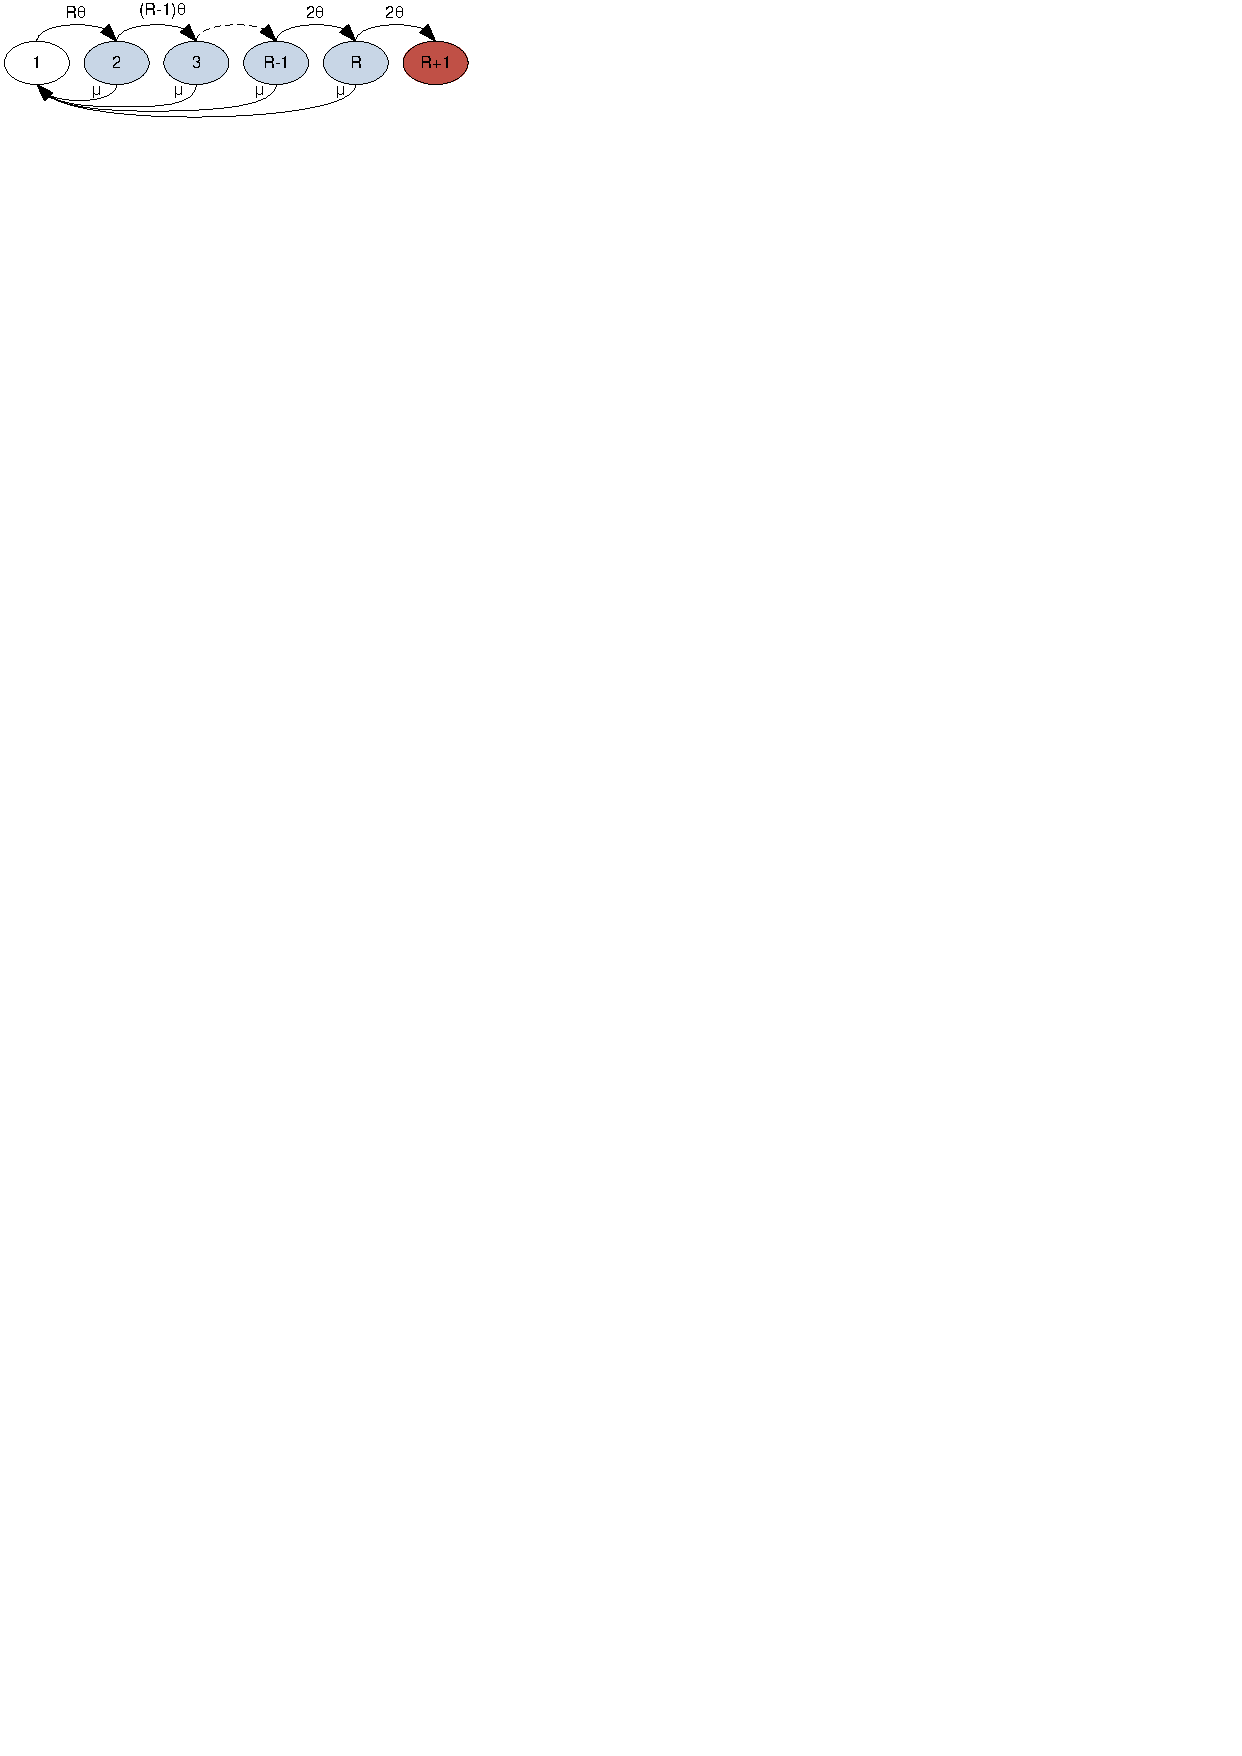
\includegraphics[clip=true, viewport=0.0cm 27.5cm 8.0cm 30.0cm, width=0.7\columnwidth]{inifinite_network_chain}
 \caption{Markov chain modeling object replica number for an infinite network size}
 \label{fig_other_markov_chain}
\end{figure}

The model has $R+1$ states and is in state $k$ when $R+1-k$ replicas are alive in the network. The system is, therefore, in state $1$ when all replicas are present and in state $R+1$ when no replicas are present. The authors assume that all objects are inserted into the network with $R$ replicas, i.e. enter the network in state 1. The initial state is colored white in Figure \ref{fig_other_markov_chain}. If the node departure rate under steady state is $\theta$ and there are $r$ replicas present in the network, the replica departure rate under steady state is $r\theta$.

It is assumed that the Markov chain can lose a single replica at any time instance and that a repair mechanism exists. When repair occurs, at a rate of $\mu = 1/T_{\textrm{repair}}$, all replicas are replaced and the object is as healthy as it was when it was initially stored. When all replicas are lost, the chain enters state $R+1$ and is said to be ``absorbed''. The absorbtion state is coloured dark.

Our paper improves on the work by Wu, Tian and Ng \cite{replication_article} in two ways: firstly, the model is extended to take into account a finite network size. The fact that there might not be sufficient nodes to replicate the data on when objects are stored or when the repair mechanism activates. Secondly, our model unifies the cases with and without repair, to produce a single model where the effects of both might be evaluated. When our model is used with larger average network sizes, expected object lifetimes converge to those shown in the work by Wu, Tian and Ng, using their two separate models.

\section{The model}
\label{model}

In order to model the effects of a finite network size on the lifetime of an object, the continuous time Markov chain model introduced in Section \ref{related_work} is expanded by adding a second parameter to every state, namely the network size. This effectively adds another dimension to the Markov chain. The resulting Markov chain is shown in Figure \ref{fig_markov_chain}.

\begin{figure}[htbp]
 \centering
 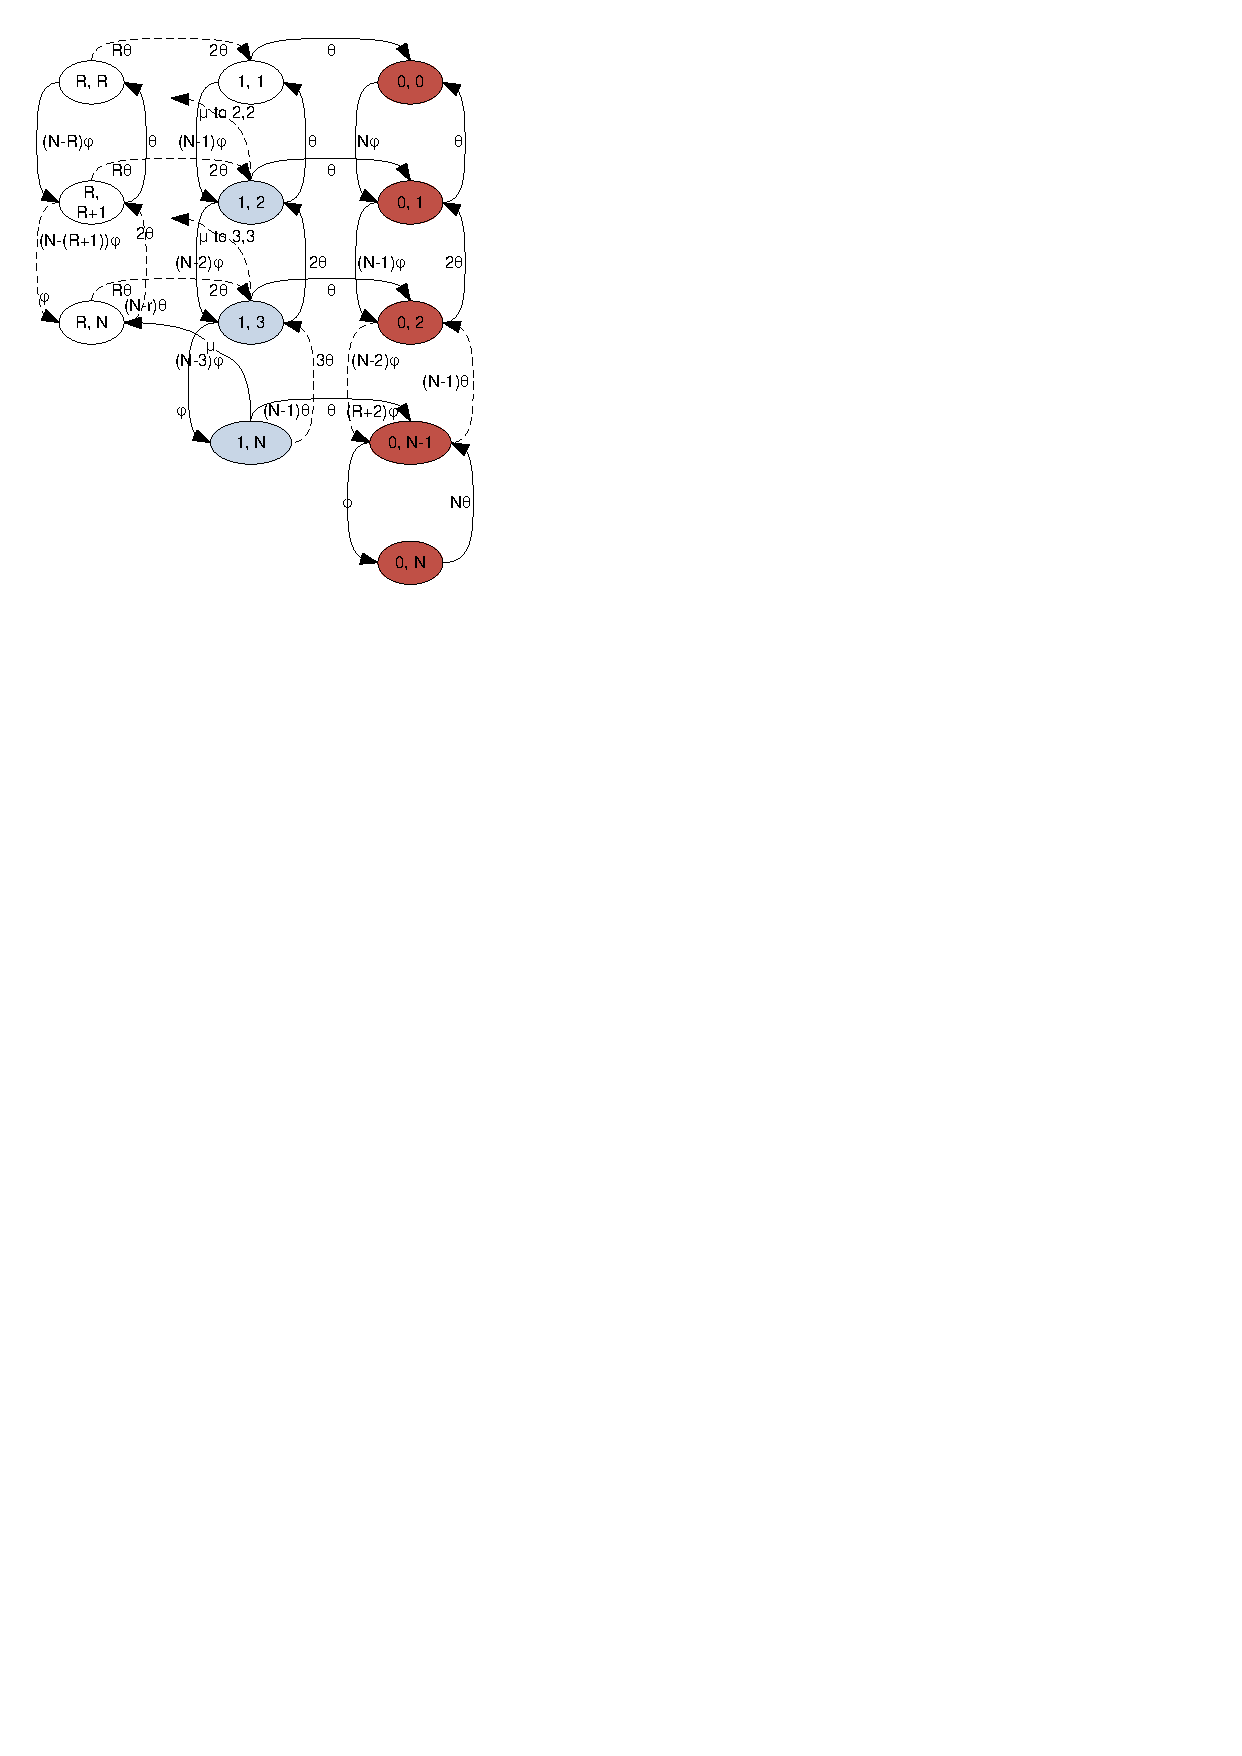
\includegraphics[clip=true, viewport=0.5cm 19.5cm 8.5cm 29.5cm, width=0.7\columnwidth]{Markov_chain_repair_compact}
 \caption{Markov chain modeling object replica number as well as network size}
 \label{fig_markov_chain}
\end{figure}

%Explain transient and absorbtion states here somewhere.

The dual parameter states can be seen in the Markov chain in Figure \ref{fig_markov_chain}. Every state is a tuple of the form \verb.(replicas,nodes).. Where $R$ is the required number of object replicas and $N$ is the maximum number of nodes in the network. It is assumed that $R$ replicas are always stored in the network, if sufficient space is available. If the number of nodes currently in the network $n$ are fewer than the required number of replicas ($n < R$), only $n$ replicas are stored. The initial states of the Markov chain are therefore all the states ($R,n$) as well as all the states ($n,n$), for $n < R$. There are therefore $N$ initial states, one for every possible network size. The initial state is the initial network size that an object is placed in.

If there are no more replicas in the network, an object cannot be repaired and the Markov chains remains in the set of states ($0,n$). These are said to be the absorbing states of the Markov chain and there exists $N - R + 1$ absorbing states in the model presented here. All other states out of which transition is possible are said to be transient states. When these states exist, the Markov chain is said to be absorbing. It can be shown that if sets of transient and absorbing states exist, the system will always end up in the absorbing states \cite{grinstead1997introduction_probability}. The time to absorbtion can be calculated, which in the case of object storage means the time when no more objects exist in the network.

\subsection{State transition rates}

There are four types of state transitions possible in the Markov model presented here:
%
\begin{enumerate}
\item A node that contains a replica departs the network.
\item A node that does not contain a replica departs the network.
\item A node joins the network.
\item An object is repaired.
\end{enumerate}

%In a continous Markov chain we define delta small enough so only one event can occur at any point in time

\begin{figure}[htbp]
 \centering
 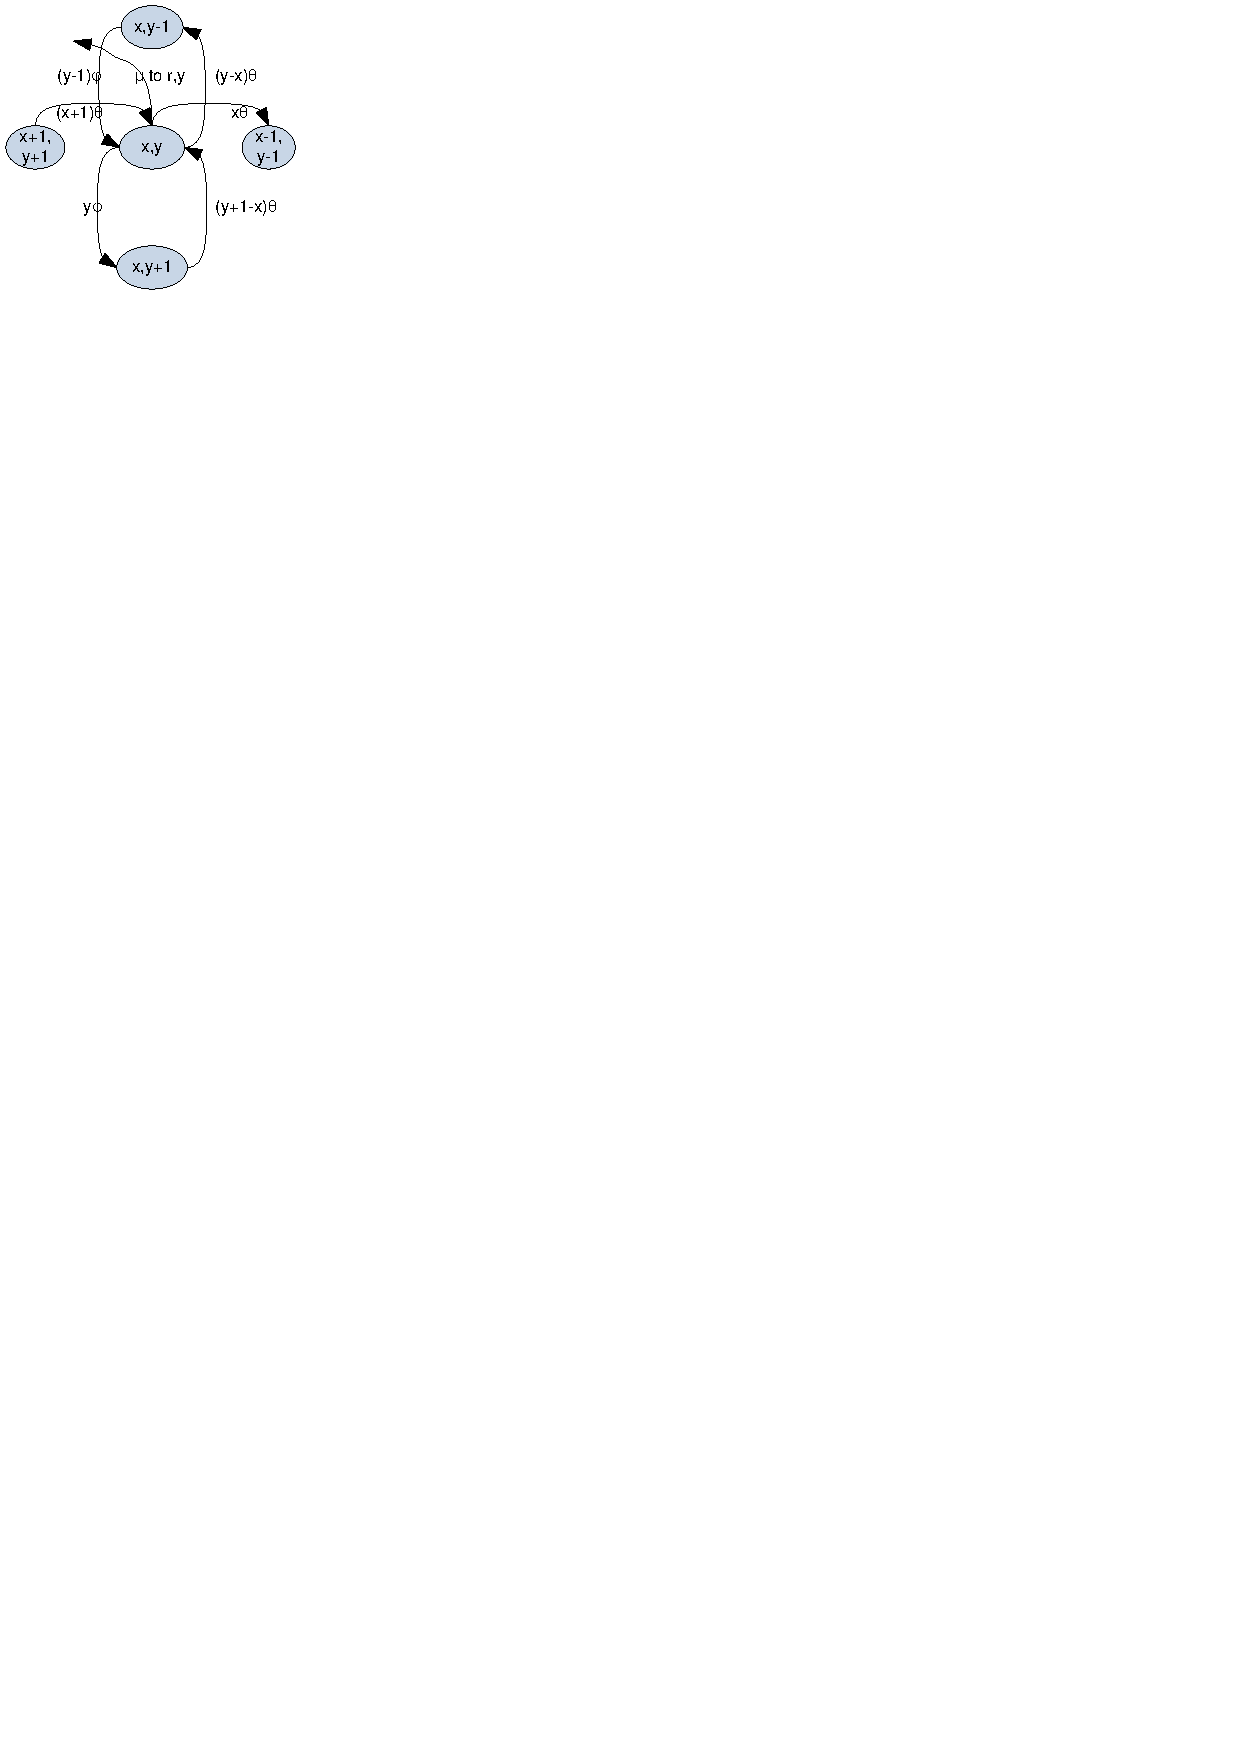
\includegraphics[clip=true, viewport=0.0cm 24.5cm 5.0cm 30cm, width=0.6\columnwidth]{Markov_example}
 \caption{Markov chain modeling object replica number as well as network size}
 \label{fig_markov_example}
\end{figure}

State transitions can be explained by the example in Figure \ref{fig_markov_example}. The figure shows all state transitions relative to the centre state ($i,k$). For the purposes of explanation, only transitions to and from the centre state are shown. Starting at state ($i+1,k+1$), where $i+1$ replicas and $k+1$ nodes are present. If a node that contains a replica departs the network, the system moves to state ($i,k$): one fewer replica and one fewer node.

If a node that does not contain a replica now departs from the network, the system moves from state ($i,k$) to ($i,k-1$): no fewer replicas and one fewer node. A node can join the network, which will have the model move from ($i,k-1$) to ($i,k$) and another node joining the network will move the system into state ($i,k+1$).

The periodic repair mechanism, introduced in Section \ref{related_work} is also present. With sufficient nodes available for a full repair, the system moves from state ($i,k$) to ($R,k$). When the network size is smaller than the required number of replicas, the system moves to state ($N,k$) instead.

The transitions in a continuous time Markov chain are classically characterised by the rate of moving from state $i$ to state $j$. For the dual states used in the model presented in this paper, state transition rates are characterised by moving from state $i k$ to state $j l$, where $i$ is the number of replicas in the current state, $k$ the number of nodes in the current state, $j$ the number of replicas in the next state, and $l$ the number of nodes in the next state. Every state transition rate can then be expressed as a dual state transition equation.

Let $\theta$ be the departure rate of nodes under steady state. For a current state of $i$ replicas, the departure rate of nodes containing replicas from the network is $i\theta$. This transition can be expressed in terms of the dual state transition equation:
%
\begin{equation} \label{eq_rep_left}
    p(i k,j l)_{(\textrm{replica left})} = i\theta,\quad\textrm{for}\quad j = i - 1,\quad l = k - 1,
\end{equation}
%
where the next state contains one fewer replica and one fewer node than the current state.

The departure rate of nodes not containing replicas is the difference between the number of nodes currently in the network $k$ and the number of replicas currently in the network $i$. The departure rate is then $(k - i)\theta$ and the transition is given by
%
\begin{equation} \label{eq_node_left}
    p(i k,j l)_{(\textrm{node left})} = (k - i)\theta,\quad\textrm{for}\quad j = i,\quad l = k - 1,
\end{equation}
%
where the next state contains one fewer node, but the same number of replicas as the current state.

The Markov model assumes the presence of a finite sized network, with some maximum number of nodes $N$. Let $\phi$ be the arrival rate of peers under steady state. The departure rate of nodes from the network is dependant on the number of nodes in the network. Similarly, if a maximum network size is assumed, the arrival rate of nodes in the network is dependant on the number of nodes \emph{not} in the network.

This creates a symmetry between the network departure and arrival rates, which creates a ``force'' in the Markov model that pushes the network to some average network size, which is the ratio of $\theta$ to $\phi$. The presence of forces that pushes the network to some average network size is required to model a steady state network.

The arrival rate of nodes can thus be modelled as $(N - k)\phi$, the product of a single node arrival rate and the number of nodes not currently in the network, as given by
%
\begin{equation} \label{eq_node_arrived}
    p(i k,j l)_{(\textrm{node arrived})} = (N - k)\phi,\quad\textrm{for}\quad j = i,\quad l = k + 1,
\end{equation}
%
where the next state contains one more node, but the same number of replicas as the current state.

%Perhaps add some graphs here to show how node departure and arrival rate change with changes in network size. Show a graph or equation that will show the trend towards a single average. Perhaps use something like the rate difference to show force towards the centre.

$N$ should be chosen sufficiently large, compared to the average network size $\tilde{n}$, to ensure that the probability of the network model ever reaching $N$ is vanishingly small. What constitutes a sufficiently large maximum network size will be evident from the results presented in Section \ref{results}. This requires that the ratios of $\theta$ to $\phi$ be chosen to produce a network with an average network size much smaller than $N$.

For the network to be in steady state, the mean arrival rate of nodes must equal the mean departure rate of nodes, which gives
%
\begin{equation}
    (N - \tilde{n})\phi = \tilde{n}\theta.\label{eq_phi_theta_ratio}
\end{equation}

Making $\phi$ the subject of Equation \eqref{eq_phi_theta_ratio} gives
%
\begin{equation}
    \phi = \frac{\tilde{n}\theta}{N - \tilde{n}},\label{eq_phi}
\end{equation}
%
which provides a value for $\phi$ that will produce a network with the desired average network size, for a given $\theta$ and $N$.

As stated earlier, a periodic repair mechanism is assumed. It is assumed that this mechanism repairs objects once every $T_{\textrm{repair}}$ time or at a rate of $\mu = 1/T_{\textrm{repair}}$, where the transition rate equation is given by
%
\begin{equation} \label{eq_repair}
    p(i k,j l)_{(\textrm{repair})} = \mu,\quad\textrm{for}\quad j = \min(R, l),\quad l = k,\quad i \neq j.
\end{equation}
%
The number of replicas in the next state is either equal to the required number of replicas or the current number of nodes, whichever one is smallest, and the number of nodes remain the same as in the current state. When no replicas are missing, no repair occurs.

No transitions other than the ones described above can occur in the presented Markov model, therefore $p(i k,j l) = 0$ for all other state transitions.

\subsection{Node departure rate}

The node departure rate $\theta$ can be calculated from the lifetime distributions of the nodes in the network. As in the related work discussed in Section \ref{related_work}, all node lifetimes are assumed to be statistically independent and exponentially distributed with the cumulative density function (CDF) given by
%
\begin{equation} \label{exp_dist}
    F(x) = 1 - e^{-\lambda x},\quad\textrm{for}\quad \lambda > 0.
\end{equation}
%
The exponential distribution is characterised by the single ``rate'' parameter $\lambda$.

The departure rate of nodes correspond to the failure rate (also called the hazard rate) of the node lifetime distribution \cite{rausand2004systemreliability}. An advantage of the exponential distribution is its ``memoryless'' property, which has a constant failure rate $h = \lambda$ \cite{rausand2004systemreliability}. The exponential distribution is the only distribution with a constant failure rate. Node lifetimes modelled with other distributions will have to take into account the variability of the failure rate as a function of the node lifetime $h(x)$. For nodes with exponential lifetime distributions, the node departure rate is therefore $\theta = \lambda$.

\subsection{Number of states}

The Markov model presented in this paper possesses a large number of states. To calculate the total number of states, two cases are identified. The total number of states is the sum of the two cases. The first case where the number of nodes in the network is greater or equal to the required number of replicas $k \geq R$. For every possible network size in this group, there are $R$ states and $N - R + 1$ possible network sizes. From this it is evident that there are $(N - R + 1)R$ of these states.

The second case is where the number of nodes in the network is fewer than the required number of replicas. For every possible network size in this case, the number of states are equal to the number of nodes in the network, going from $R-1$ to 1.

The total number of states is the sum the two cases and given by
%
\begin{align}
       S & = R(N - R + 1) + \sum_{x=1}^{R-1} x\label{eq_states_num_init}\\
         & = R(N - R + 1) + 0.5 (R - 1) R\notag\\
         & = 0.5 R (2 N - R + 1), \quad\textrm{where}\quad N \geq R. \label{eq_states_num_ans}
\end{align}

If, for example, a small network of 500 nodes with objects each having 10 replicas is modeled, the resulting Markov chain contains 4955 states. The large number of states makes a closed form solution to the object lifetime problem intractable. Fortunately, numerical methods can be used to calculate object lifetimes for given numbers of replicas and maximum node sizes.

\subsection{Calculating object lifetimes}

Since each element in the transitional rates matrix is a rate, the sum of all the elements in a single row of the rates matrix gives the rate of moving from that state to any other state. The inverse of this rate is the expected time $t_i$ the Markov chain spends in state $i$, given by
%
\begin{equation} \label{eq_markov_rates}
    t_i = \left(\sum_{j} p_{i, j}\right)^{-1}.
\end{equation}

In a Markov chain the sum of all rows in the transitional rates matrix \textbf{P} must equal one, where \textbf{P} is the transitional rates matrix containing the rates: $p(i k,j l)_{(\textrm{replica left})}$, $p(i k,j l)_{(\textrm{node left})}$, $p(i k,j l)_{(\textrm{node arrived})}$ and $p(i k,j l)_{(\textrm{repair})}$ presented earlier. For an embedded Markov chain, this result is achieved by normalising each row in the transitional rates matrix to produce the normalised transitional rates matrix \textbf{\^{P}}, where each row in the matrix must satisfy
%
\begin{equation} \label{eq_markov_sum}
    \sum_{j} \hat{p}_{i, j} = 1.
\end{equation}

Using $t_i$, the expected time spent in state $i$, \textbf{\^{P}} is produced by
%
\begin{equation} \label{eq_markov_normalisation}
    \hat{p}_{i, j} = p_{i, j} t_i.
\end{equation}

Object lifetime can be calculated by calculating the expected time to absorbtion of the embedded continuous time Markov chain. To do this, the normalised transitional rates matrix is partitioned into the form
%
\begin{equation} \label{matrix_partition}
    \textbf{\^{P}} = \left[\begin{array}{c|c}
                   \textbf{Q} & \textbf{R} \\
                   \hline
                   \textbf{0} & \textbf{I}
                 \end{array}\right].
\end{equation}
%
Every state transition can be considered a discrete event, which allows for the continuous time Markov chain to be embedded. This allows for theory from discrete time Markov chains to be used, with the exception that events are not equally spaced in time.

\textbf{\^{P}} is partitioned in such a way that all absorbing states are in the last rows and columns of \textbf{\^{P}}. Suppose there are $a$ absorbing states and $\tau$ transient states in the model. The matrix \textbf{Q} is then a $\tau\times\tau$ sub-matrix of \textbf{\^{P}} that contains all transient states. \textbf{I} is a $a \times a$ identity matrix, \textbf{0} is a $a\times\tau$ zero matrix and \textbf{R} (not to be confused with $R$) is a nonzero $\tau\times a$ matrix.

From \textbf{Q}, the fundamental matrix \textbf{N} may be calculated as \cite{grinstead1997introduction_probability}
%
\begin{equation} \label{eq_fundamental_mat}
    \textbf{N} = (\textbf{I} - \textbf{Q})^{-1}.
\end{equation}
%
Every element $n_{x,y}$ in the fundamental matrix \textbf{N} gives the expected number of times that the model is in the state $y$, if it started in the transient state $x$.

The expected time to absorbtion is then the product of the time spent in each state and the expected number of times a state will be entered, as given by
%
\begin{equation} \label{expected_lifetime}
    \textbf{E[L]} = \textbf{Nt},
\end{equation}
%
where \textbf{t} is the vector consisting of the times $t_i$ for all $i$.

\section{Model results}
\label{results}

The equations developed in Section \ref{model} were implemented in Matlab, with sweeps performed over all parameters in questions. The results of these sweeps will be shown in this section and compared to the theoretical results of related work presented in Section \ref{related_work}. For all results presented here, the following parameter values are used: a maximum network size of $N=120$, a required number of replicas of $R = 10$ and exponential node lifetime distributions with $\lambda = \theta = 1/1800$, which gives expected \emph{node} lifetimes of $1800$ seconds.

%Maybe explain where these values come from or why the were used.

\begin{figure}[htbp]
 \centering
 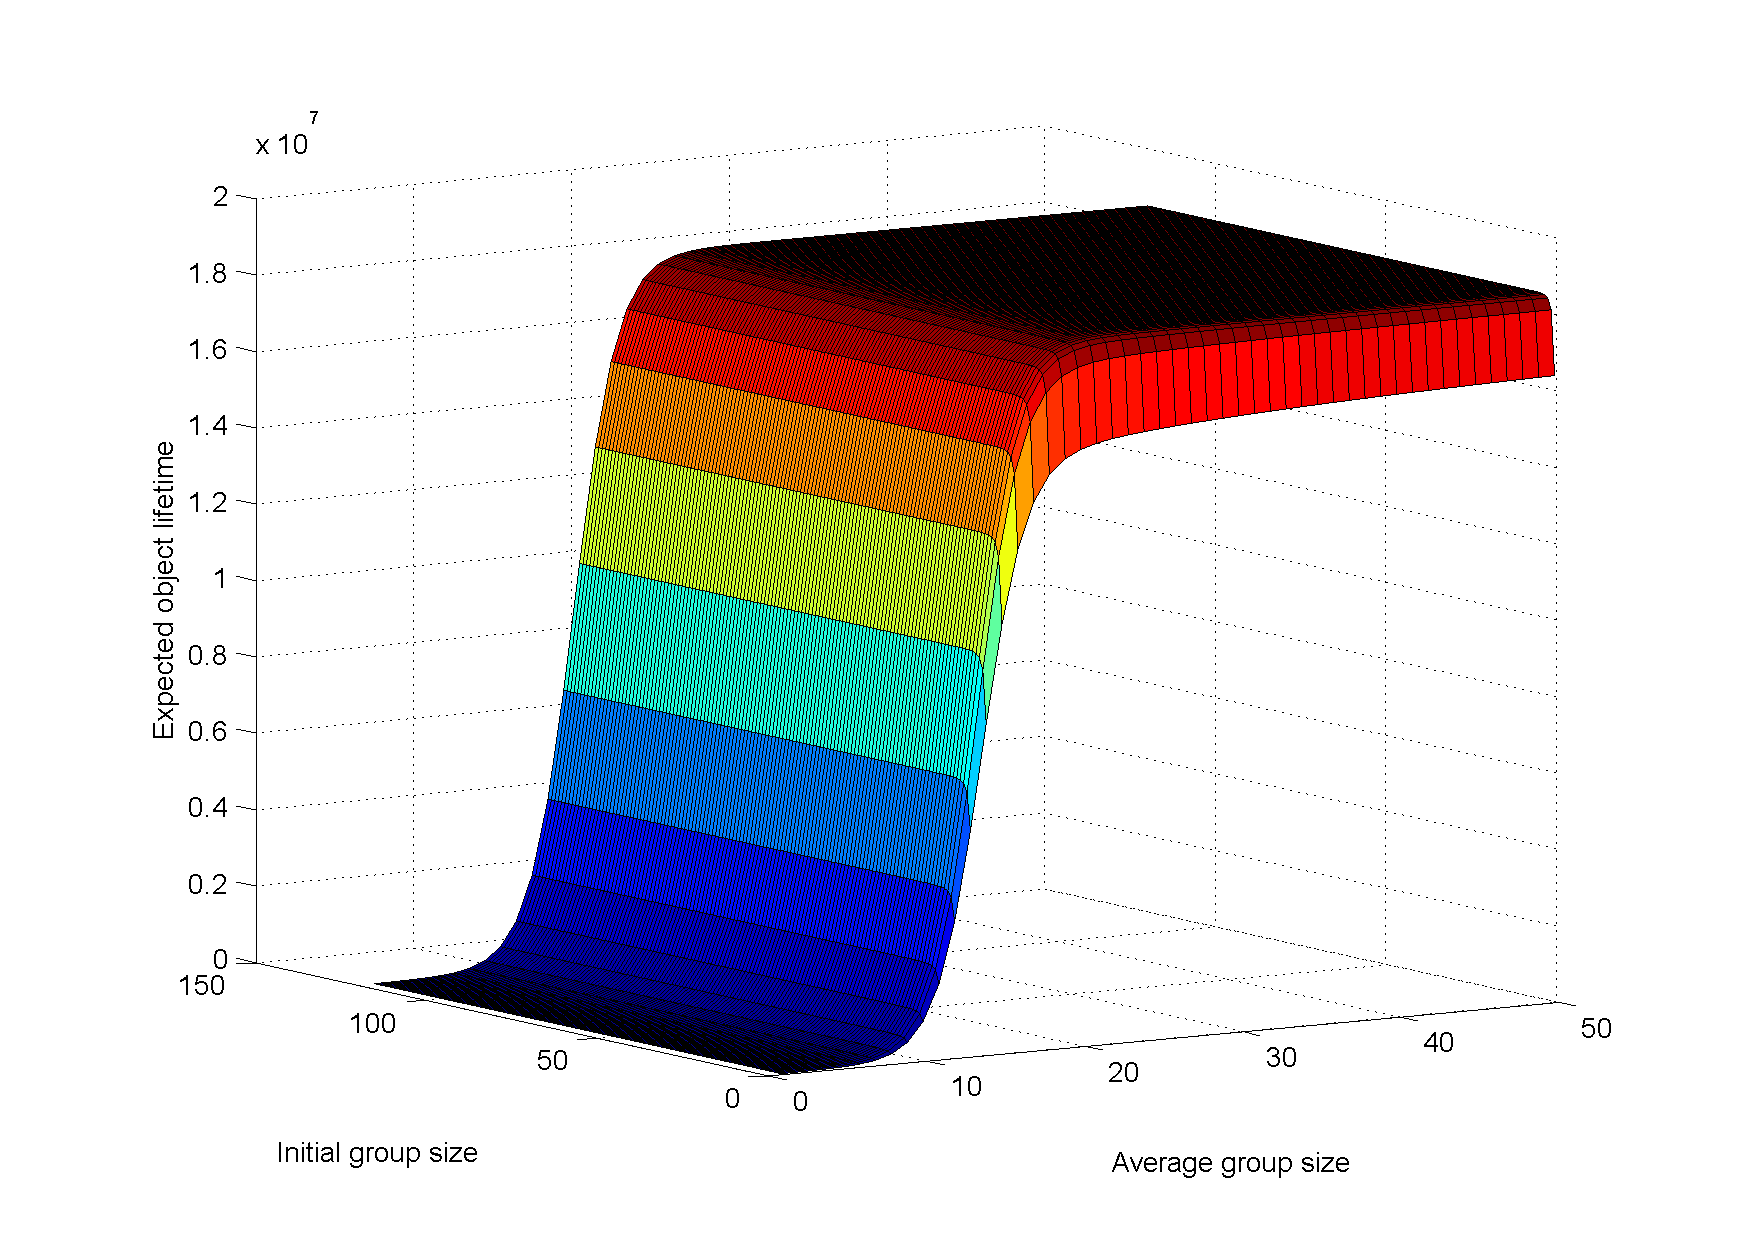
\includegraphics[clip=true, viewport=2.0cm 1.0cm 27.5cm 19.15cm, width=\columnwidth]{lifetime_av_init_groupsize}
 \caption{Surface plot of expected object lifetimes as functions of initial and average network sizes for $\mu = 1/180$.}
 \label{fig_lifetime_average_vs_initial_rep}
\end{figure}

Figure \ref{fig_lifetime_average_vs_initial} shows a surface plot of expected object lifetimes against initial and average network sizes for a repair rate of $\mu = 1/180$ (or $T_{\textrm{repair}}$ $10\%$ of the expected node lifetime). It is evident that object lifetimes decrease greatly for average network sizes smaller than 20 nodes. This is the case any time the average network size is comparable to the required number of replicas.

Figure \ref{fig_lifetime_average_vs_initial} also shows that expected object lifetimes decrease when the initial network size is smaller than the required number of replicas. The percentage decrease is studied in more depth, later in this section.

\begin{figure}[htbp]
 \centering
 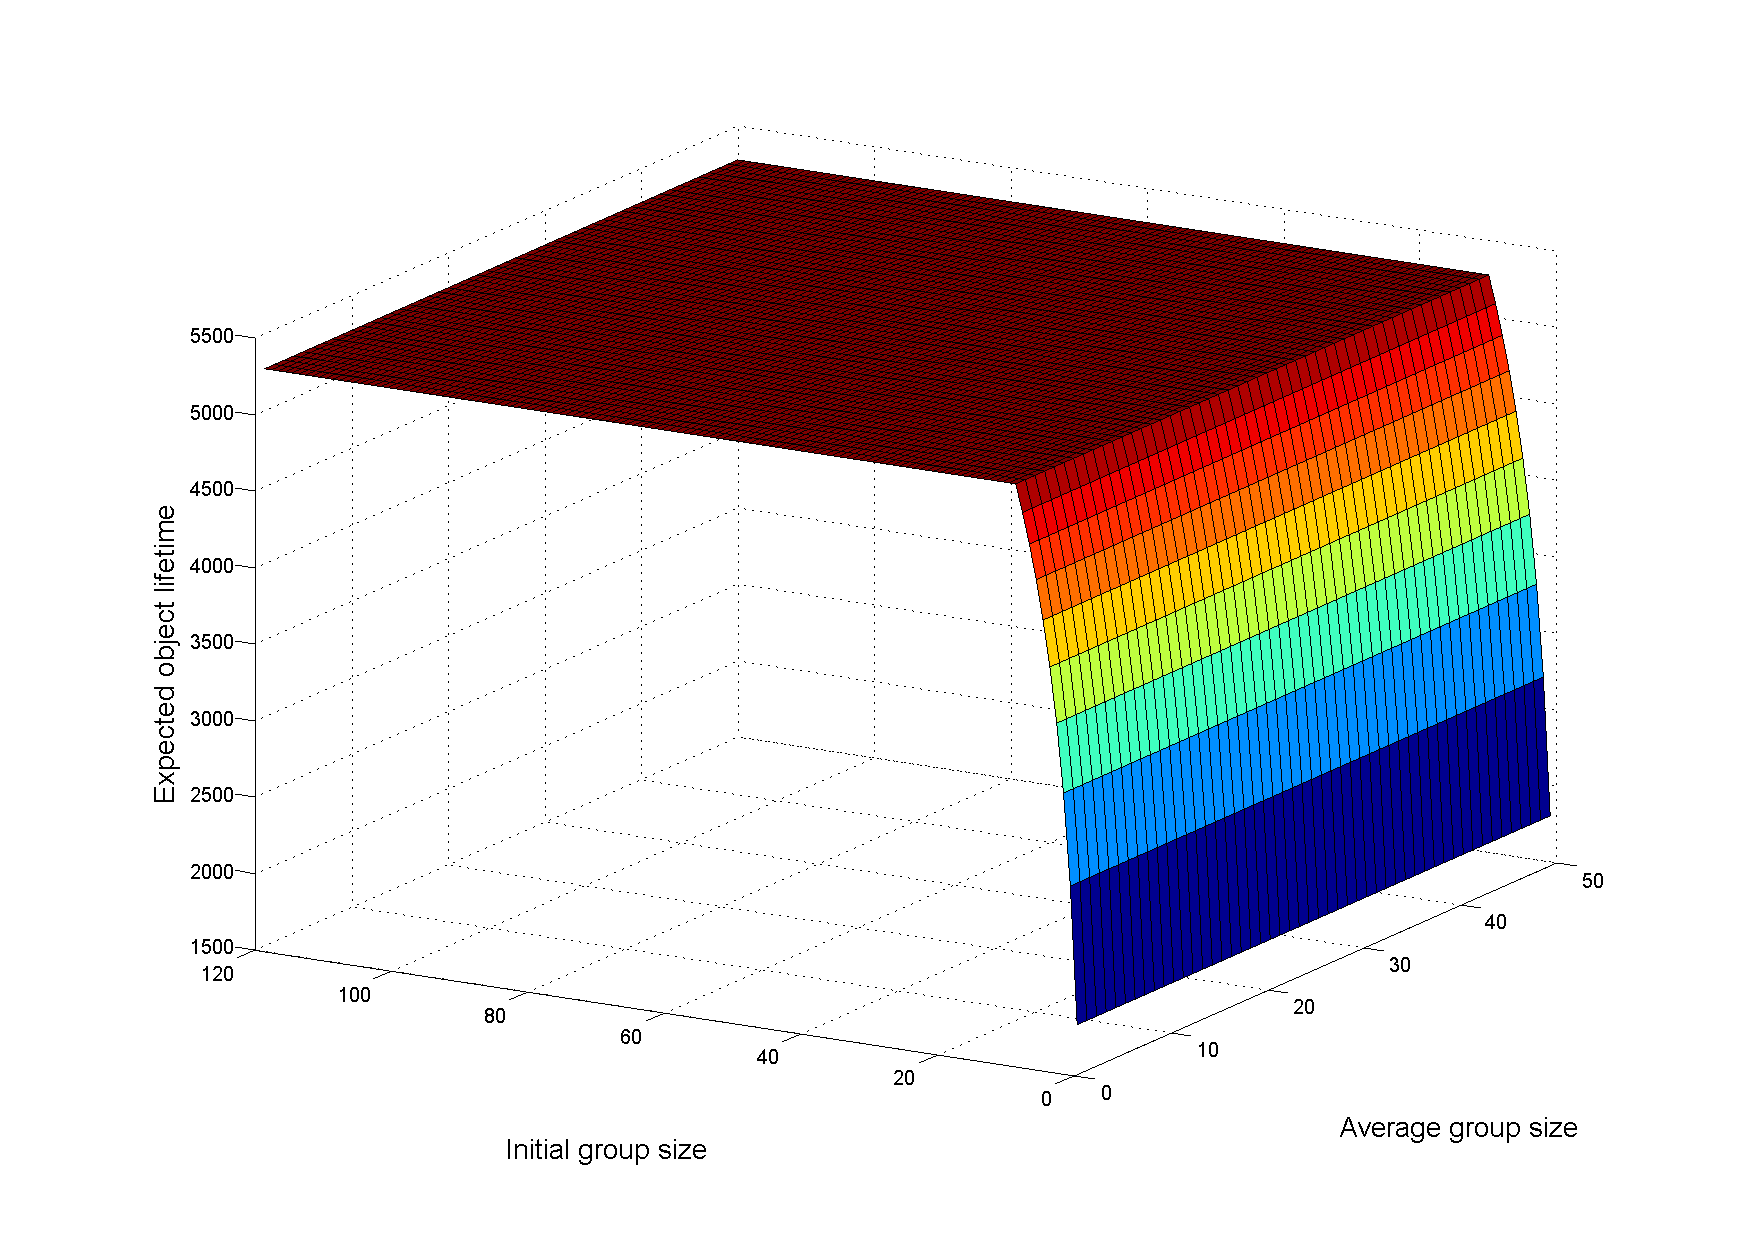
\includegraphics[clip=true, viewport=2.5cm 1.0cm 27.5cm 19.15cm, width=\columnwidth]{lifetime_av_init_groupsize_norep}
 \caption{Surface plot of expected object lifetimes as functions of initial and average network sizes for $\mu = 0$.}
 \label{fig_lifetime_average_vs_initial_norep}
\end{figure}

Figure \ref{fig_lifetime_average_vs_initial_norep} illustrates the effects of initial network size and average network size on expected object lifetime when no repair is performed. For the case of no repair, the average network size has no effect on the expected object lifetime. This result is intuitive, since an object's lifetime only depends on the lifetimes of the nodes on which it was initially placed when no repair is performed.

The initial network size, on the other hand, has a significant effect on the expected object lifetime. Object lifetimes decrease when fewer replicas than the required number of replicas can be stored.

\begin{figure}[htbp]
 \centering
 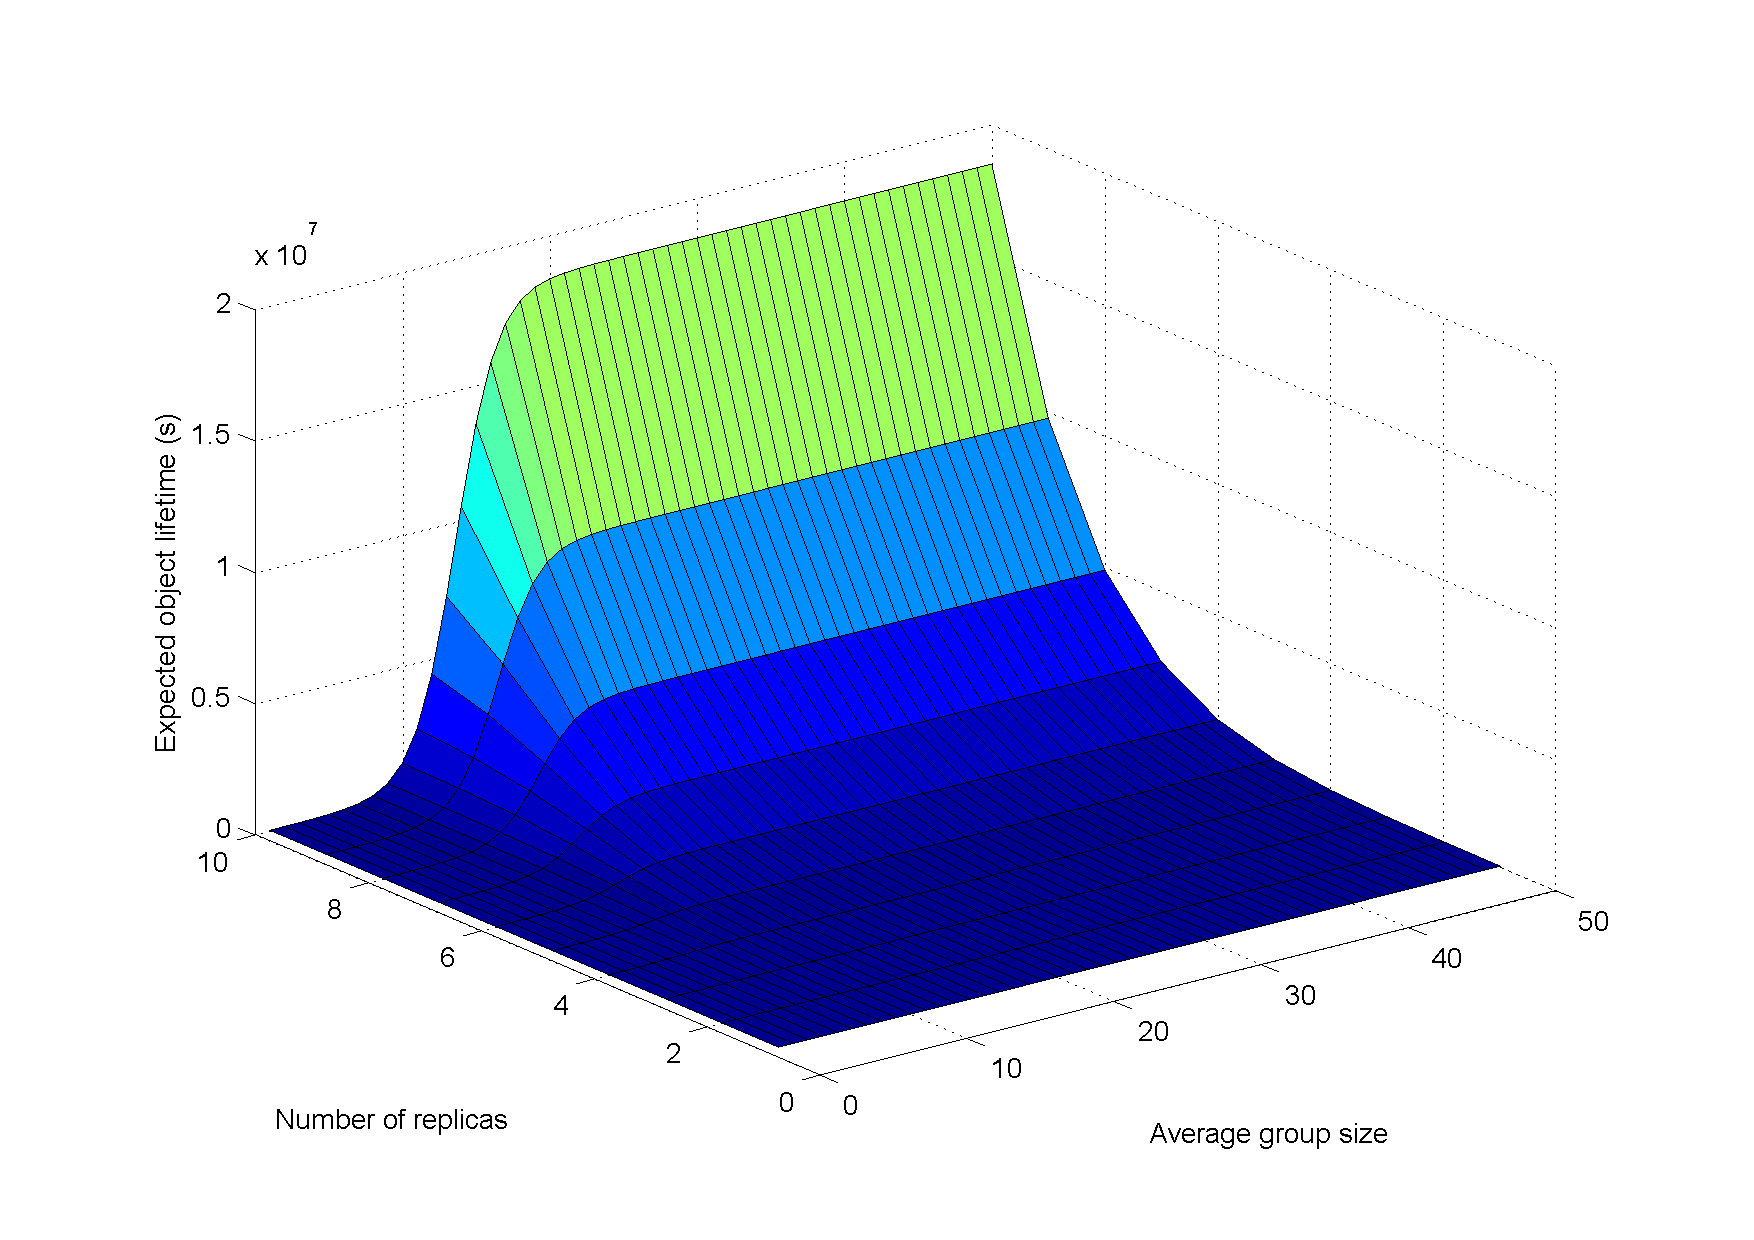
\includegraphics[clip=true, viewport=2.5cm 1.0cm 27.5cm 19.15cm, width=\columnwidth]{lifetime_replicas_av_groupsize}
 \caption{Surface plot of expected object lifetimes as functions of average network size and required number of replicas $R$ for $mu = 1/180$.}
 \label{fig_lifetime_average_vs_replicas}
\end{figure}

Figure \ref{fig_lifetime_average_vs_replicas} depicts expected object lifetime as functions of average network size and required number of replicas $R$ for a repair rate of $\mu = 1/180$. To generate this figure, $R$ is swept from 1 to 10 to illustrate the effect that an increase in the number of replicas has on the expected node lifetime. The figure shows that an increase in $R$ leads to an exponential increase in the expected object lifetime, but that this gain is limited when the average network size is small, compared to the required number of replicas.

\begin{figure}[htbp]
 \centering
 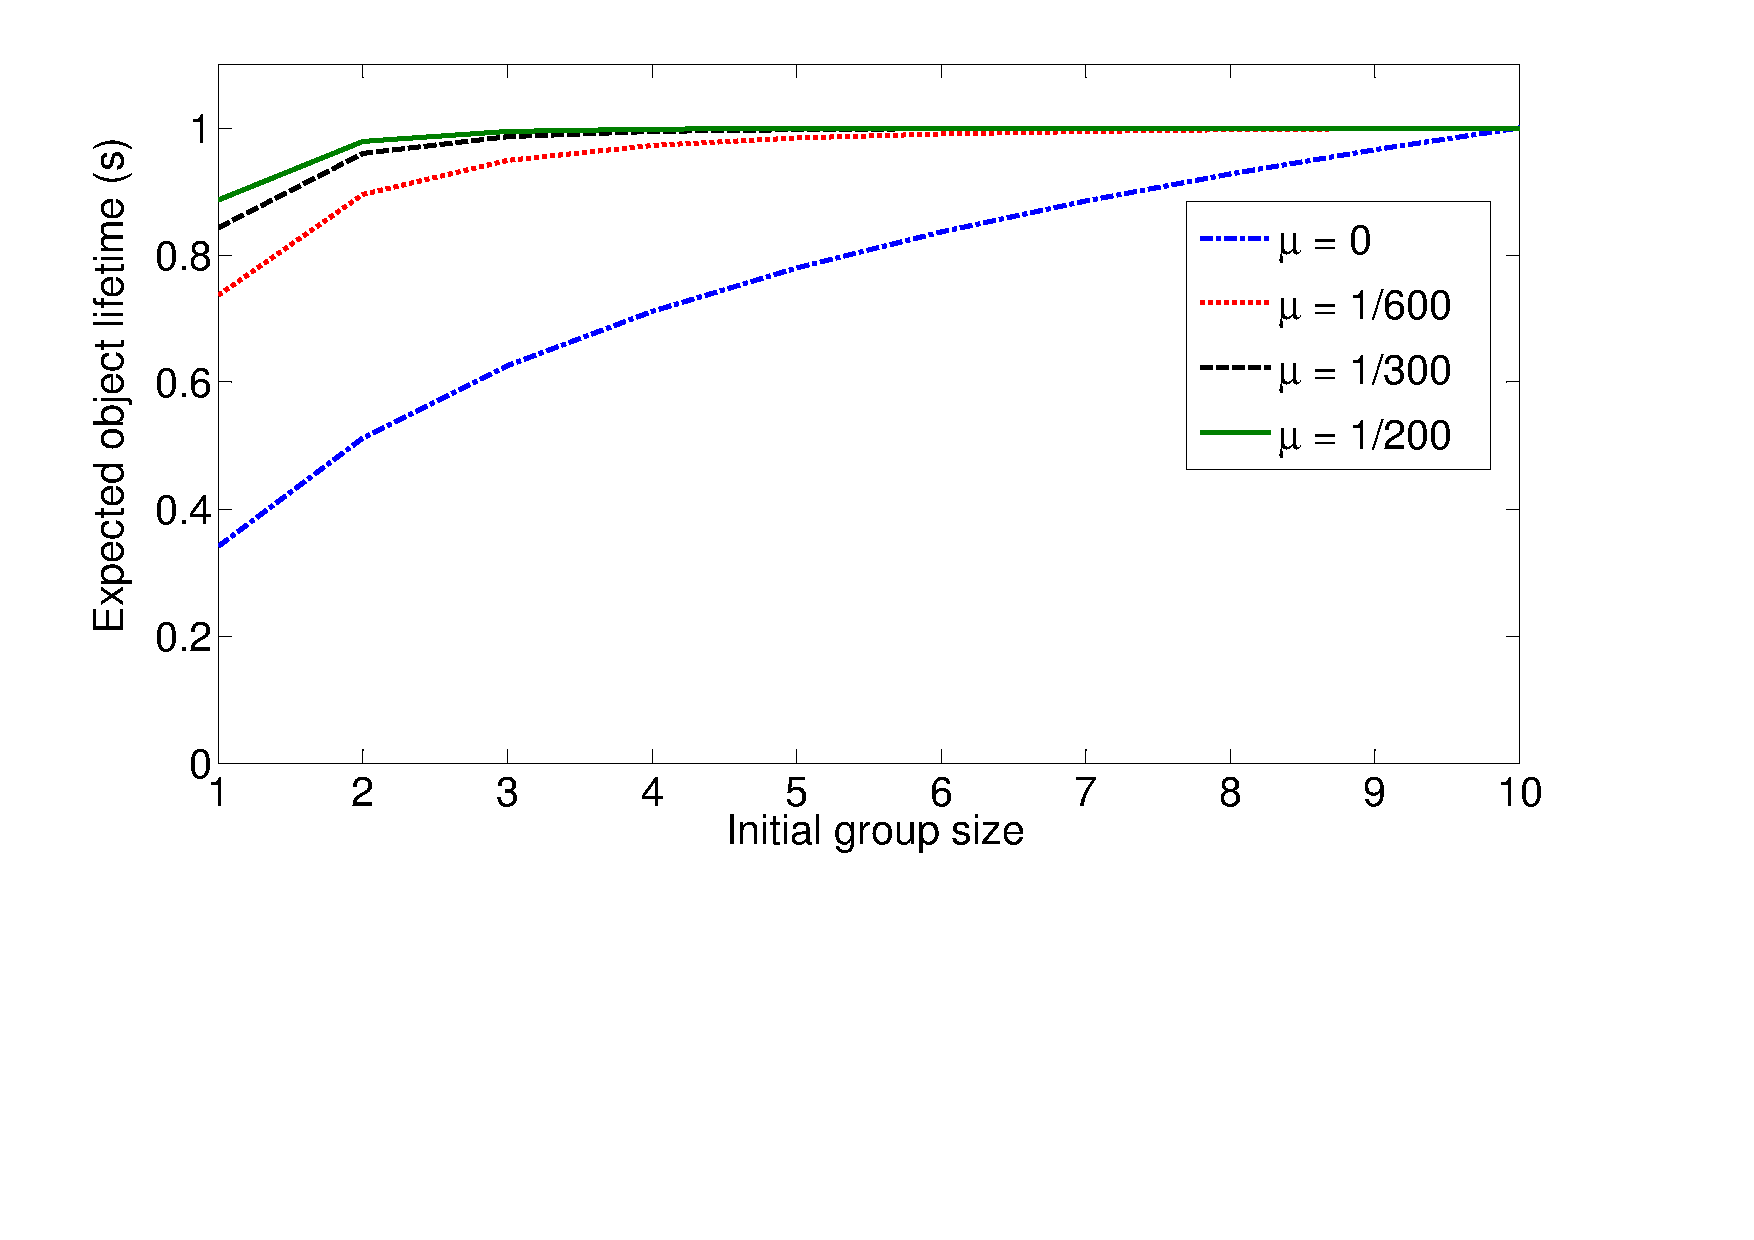
\includegraphics[clip=true, viewport=1.0cm 6.5cm 24.7cm 22.0cm, width=0.9\columnwidth]{lifetime_replication_repair}
 \caption{Comparison of the effects of different repair rates on object lifetime for initial network sizes smaller than the required number of replicas.}
 \label{fig_lifetime_replication_effect_on_initial}
\end{figure}

Figure \ref{fig_lifetime_replication_effect_on_initial} illustrates the effect various repair rates have on the object lifetime as functions of initial network size. The figure was generated with an average network size of 50 nodes. The figure shows that for higher repair rates, object lifetimes are less influenced by the case where insufficient replicas were available for storage.

This result is also intuitive. For a sufficiently large average network size, if there were insufficient nodes available in the network at the time when an object was stored, if the repair rate is high, as soon as the network size increases, the object will be repaired to the same number of replicas as every other object in the network. This would mean less dependance on initial network size.

\begin{figure}[htbp]
 \centering
 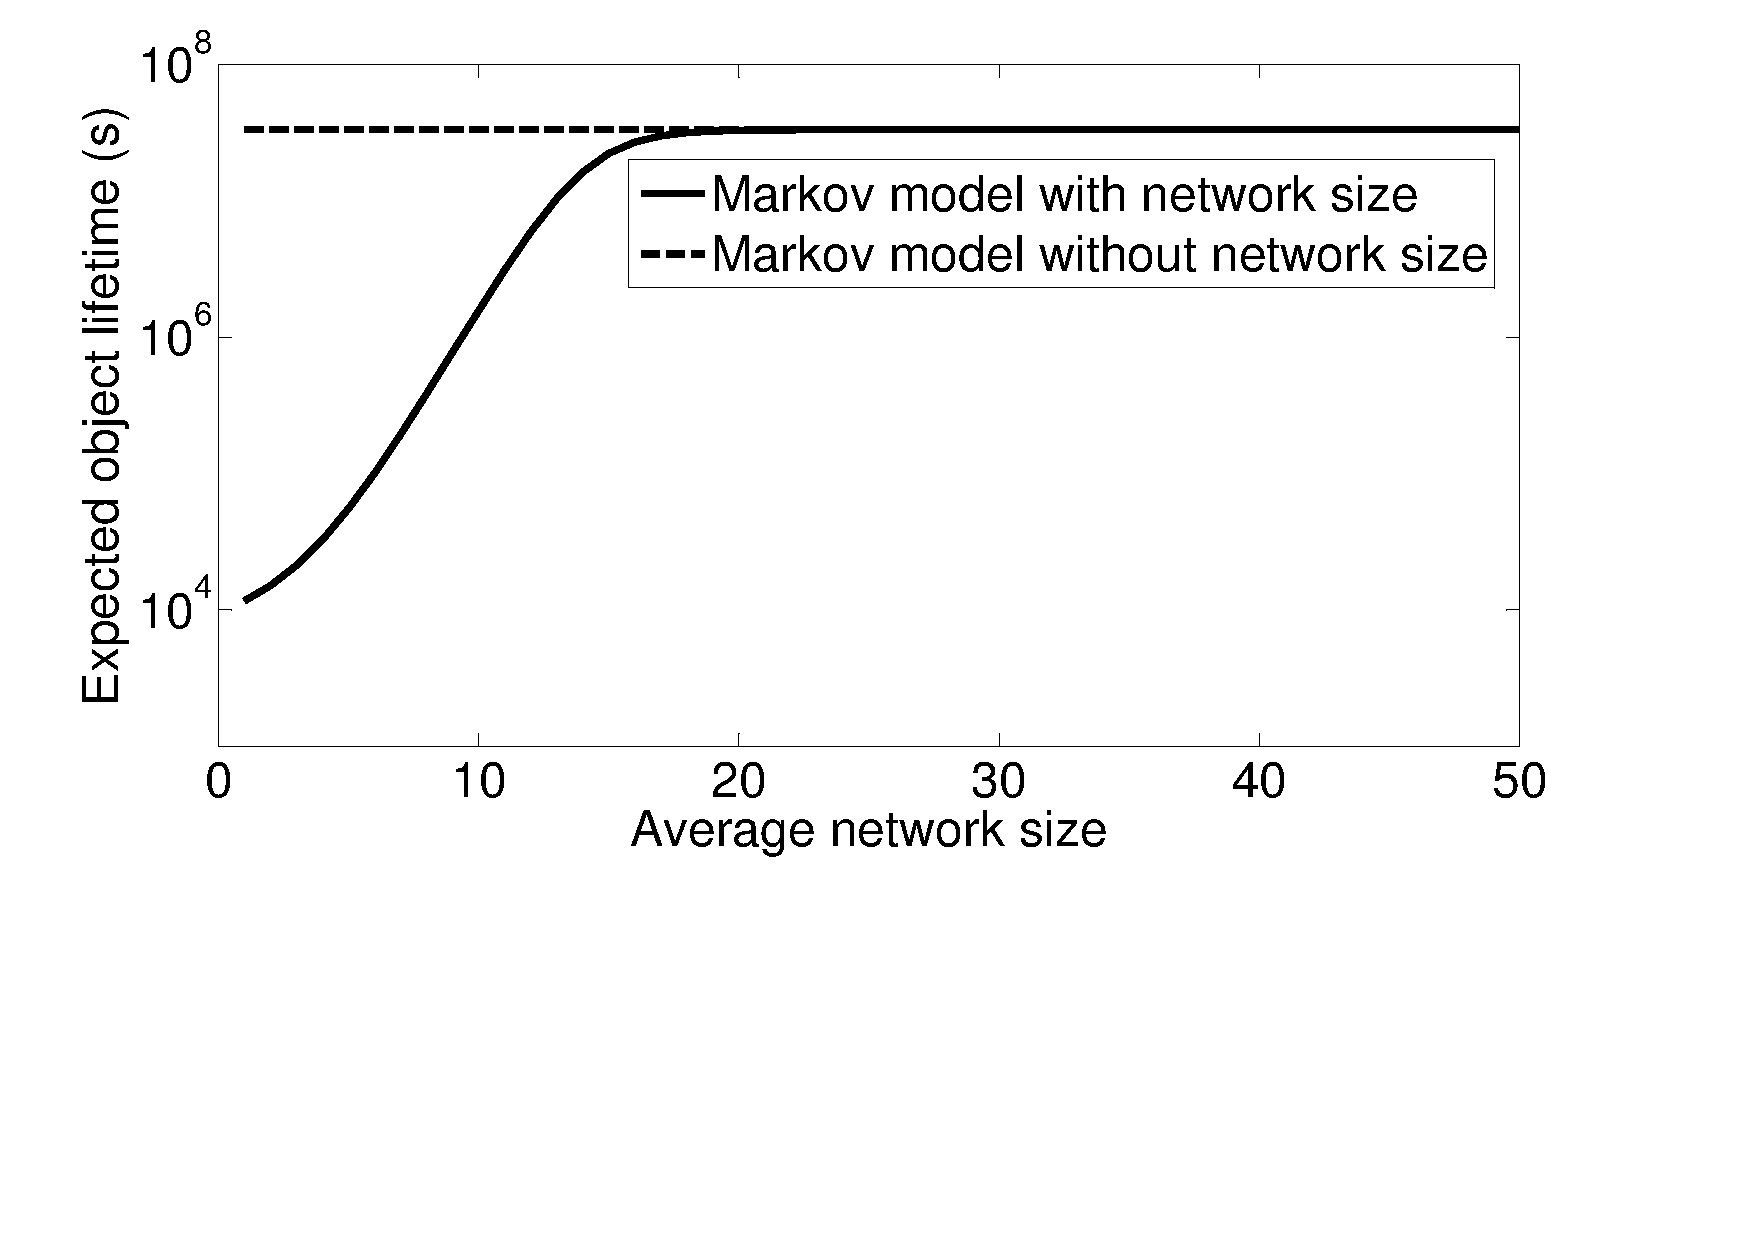
\includegraphics[clip=true, viewport=1.0cm 6.5cm 26.5cm 20.5cm, width=0.9\columnwidth]{lifetime_av_models_compare}
 \caption{Surface plot of expected object lifetimes as functions of initial and average group sizes.}
 \label{fig_lifetime_vs_other_model}
\end{figure}

Figure \ref{fig_lifetime_vs_other_model} compares the model presented in this paper with the model of Wu, Tian and Ng that assumes object repair \cite{replication_article}. For this figure, a repair rate of $\mu = 1/180$ and a required number of replicas of $R = 10$ were used. A shown, because the model by Wu, Tian and Ng does not take average network size into account (or initial network size for that matter) it cannot predict the object lifetimes correctly for average network sizes comparable to the required number of replicas.

On the other hand, a reliability test of the model presented in this paper is that for sufficiently large network sizes, the model should converge to a model that effectively assumes an infinite network size. This is also shown to be the case.

What remains is to compare the model presented in this paper with some practical results.

\section{Comparison with Pithos simulation}
\label{simulation}

To determine practical usability of the theoretical results presented in Section \ref{results}, a comparison was performed against the Pithos simulation \cite{Pithos_mmve_2011}.

%Explain the basics of Pithos 

Pithos was used to generate simulation data to compare with the theoretical model. A single group was used to allow for control over the average network size. All nodes posses exponential lifetime distributions to match the theoretical model.

``Box and whiskers plots'' are used to compare the simulation data with the theoretical model. This allows for comparisons of mean values, but also shows how the data are distributed. In the box plot, the black striped whiskers show the minima and maxima of the data sets. The lower and upper bounds of the boxes show the 25th and 75th percentile of the simulation data respectively. The horizontal lines in the boxes show the medians of the data, and the ``notches'' around the medians show the 5\% significance levels. Two medians are significantly different if their significance intervals do not overlap \cite{}.

The cross present in every box shows the simulation data mean and the solid line running through the boxes shows expected object lifetimes as predicted by the theoretical model.

\begin{figure}[htbp]
 \centering
 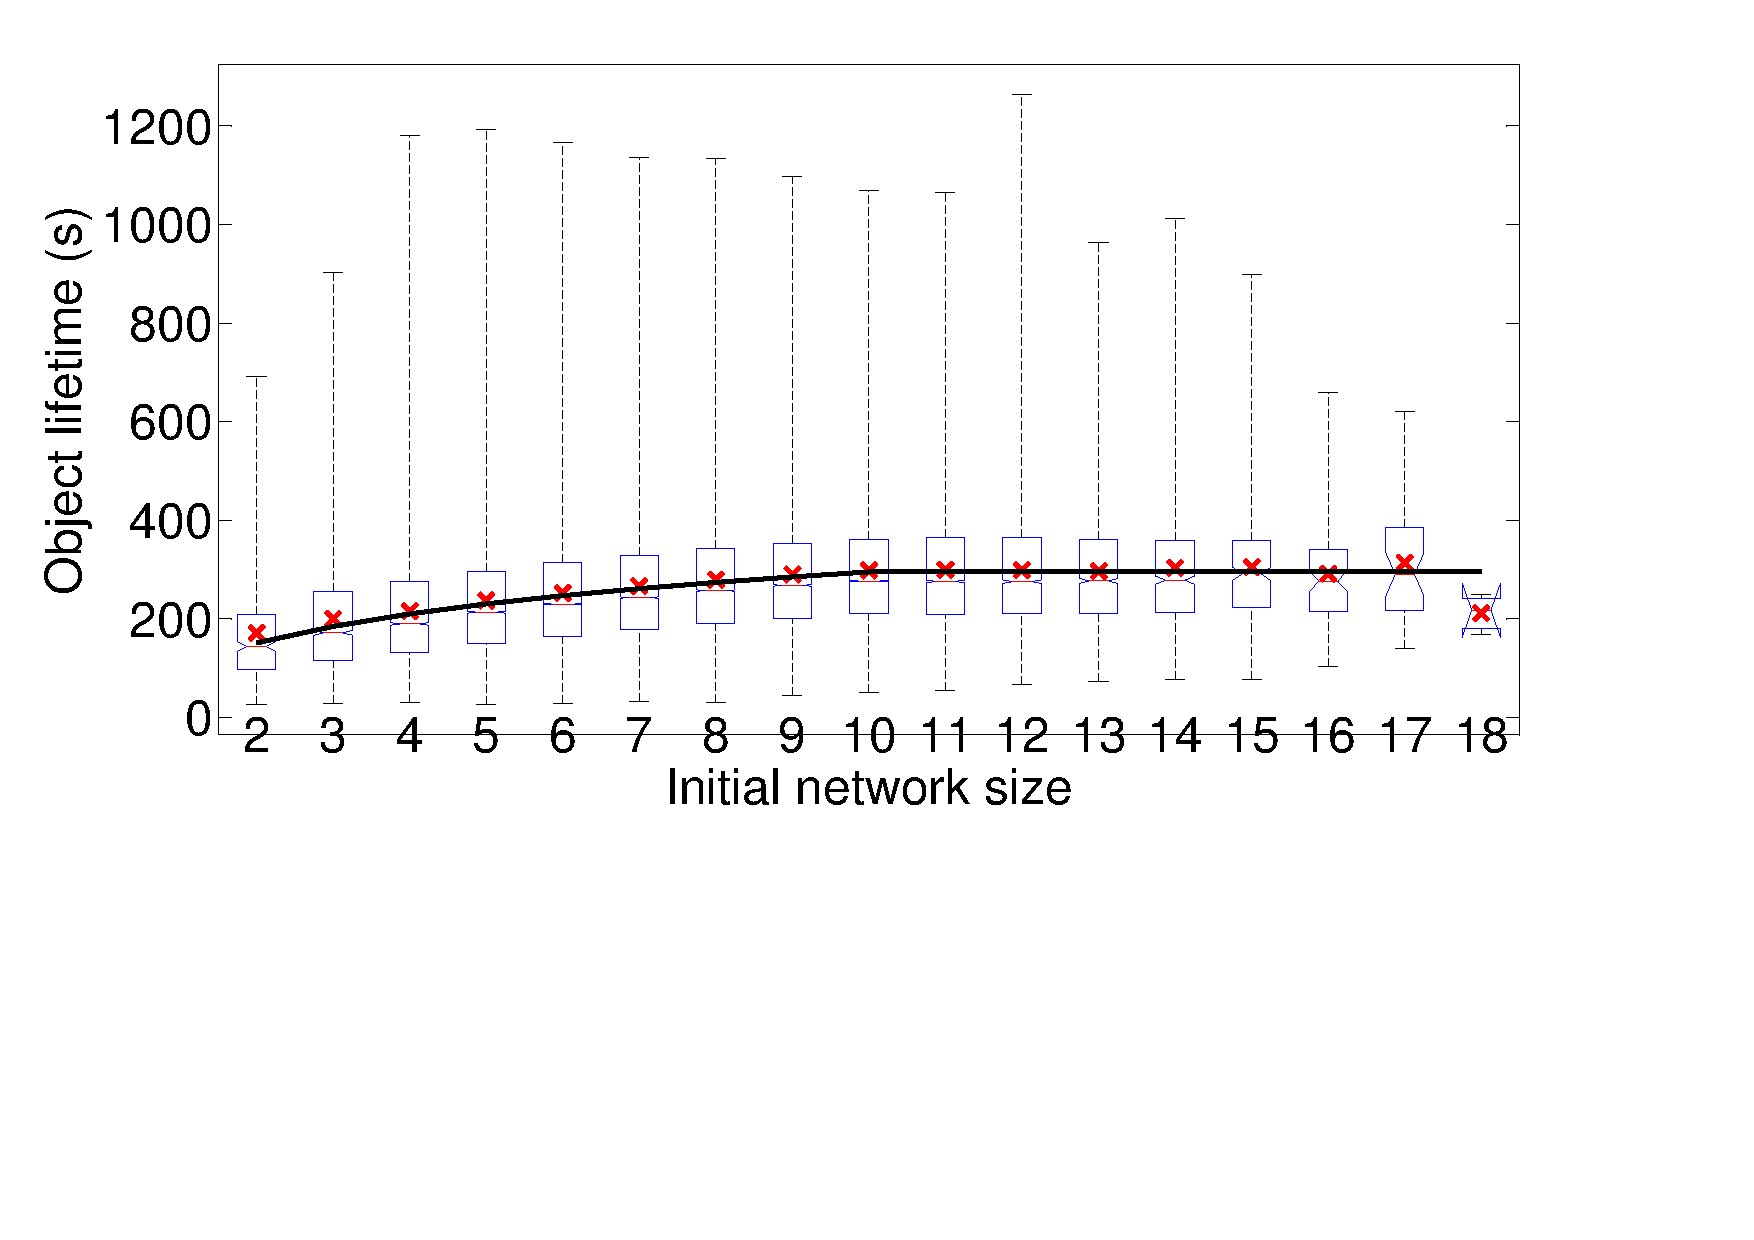
\includegraphics[clip=true, viewport=0.5cm 7.0cm 26.0cm 20.0cm, width=\columnwidth]{lifetime_simulation_model_none_100}
 \caption{Comparison of object lifetime simulation results, as a box plot, with theoretical model results for no repair, node lifetimes of $100 s$ and an average network size of 7 nodes.}
 \label{fig_lifetime_simulation_model_none_100}
\end{figure}
%
Figure \ref{fig_lifetime_simulation_model_none_100} compares the theoretical results to simulation results for the case where no repair is performed, node lifetimes are $100 s$, the number of replicas are 10 nodes and the average network size is 7 nodes.

The expected object lifetimes as predicted by the theoretical model pass through the crosses that show the simulation data means. It can, therefore, be seen that the theoretical model matches the simulation data well for the case with no repair.

\begin{figure}[htbp]
 \centering
 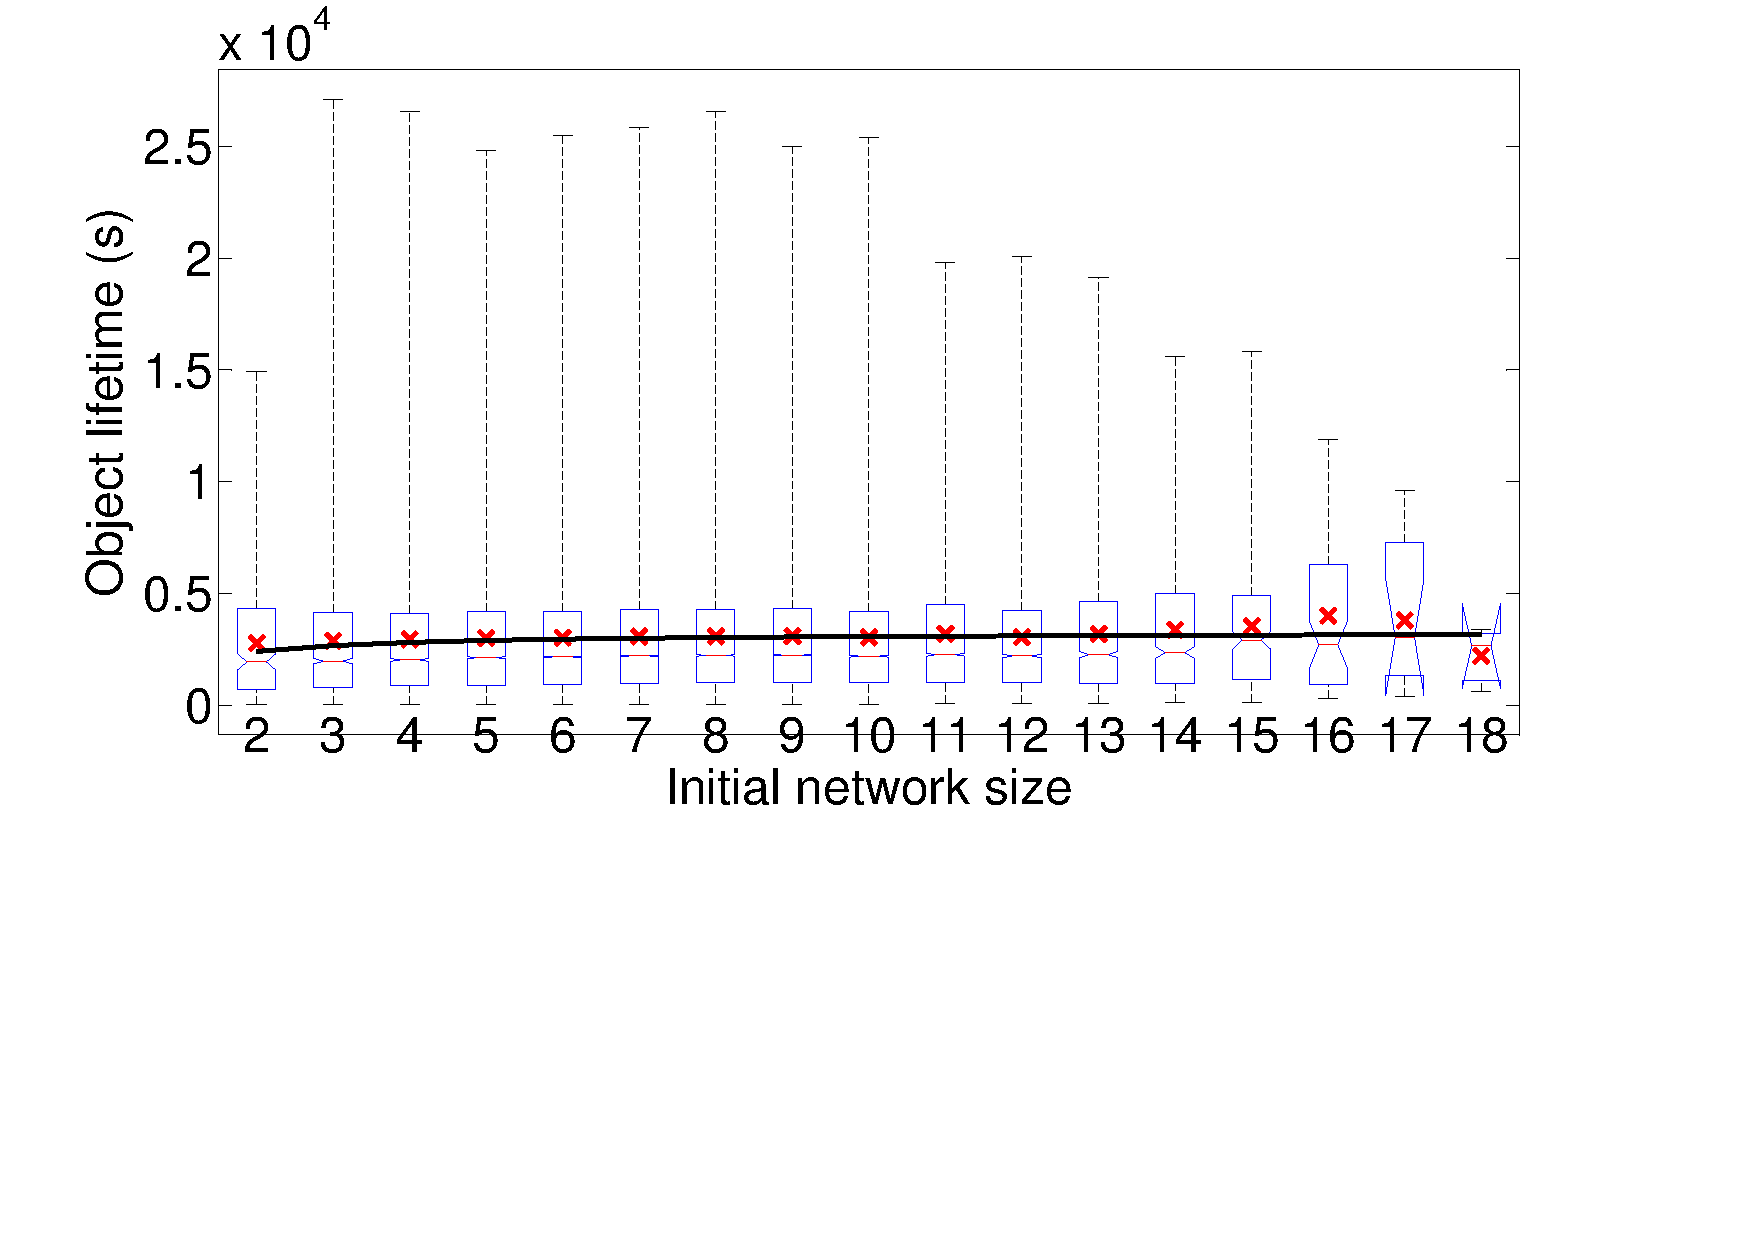
\includegraphics[clip=true, viewport=0.5cm 7.0cm 26.0cm 21cm, width=\columnwidth]{lifetime_simulation_model_20_100}
 \caption{Comparison of object lifetime simulation results, as a box plot, with theoretical model results for a repair time of $20 s$, node lifetimes of $100 s$ and an average network size of 7 nodes.}
 \label{fig_lifetime_simulation_model_20_100}
\end{figure}
%
Figure \ref{fig_lifetime_simulation_model_20_100} shows simulation data and theoretical model data for the same parameters as the previous figure, but for the case with $20 s$ repair time. A significant increase in object lifetimes can be observed. Again, the expected object lifetime as predicted by the model pass through the measured object lifetime means of the simulations.

One issue that was encountered when comparing simulation data to model data was the imperfect repair scheme used in simulation. In the simulation, every $T_{\textrm{repair}}$ time, a repair of all objects in the system is initiated. There is, however, a chance that the node that was chosen to repair an object leaves the network before the repair can complete. This reduces the effectiveness of the repair mechanism, effectively reducing the repair rate. The percentage repair successes was measured during simulation and found to be $70 \%$. All repair rates in the simulation were adjusted with this number, which successfully aligned the simulation data means with the model data means.

What is evident from all box-and-whiskers plots is the large variance and large maximum values of object lifetimes measured in the simulation. This ``heavy-tailed'' distribution is also evident when looking at the overall object lifetime distribution shown in Figure \ref{fig_object_lifetimes}. 

\begin{figure}[htbp]
 \centering
 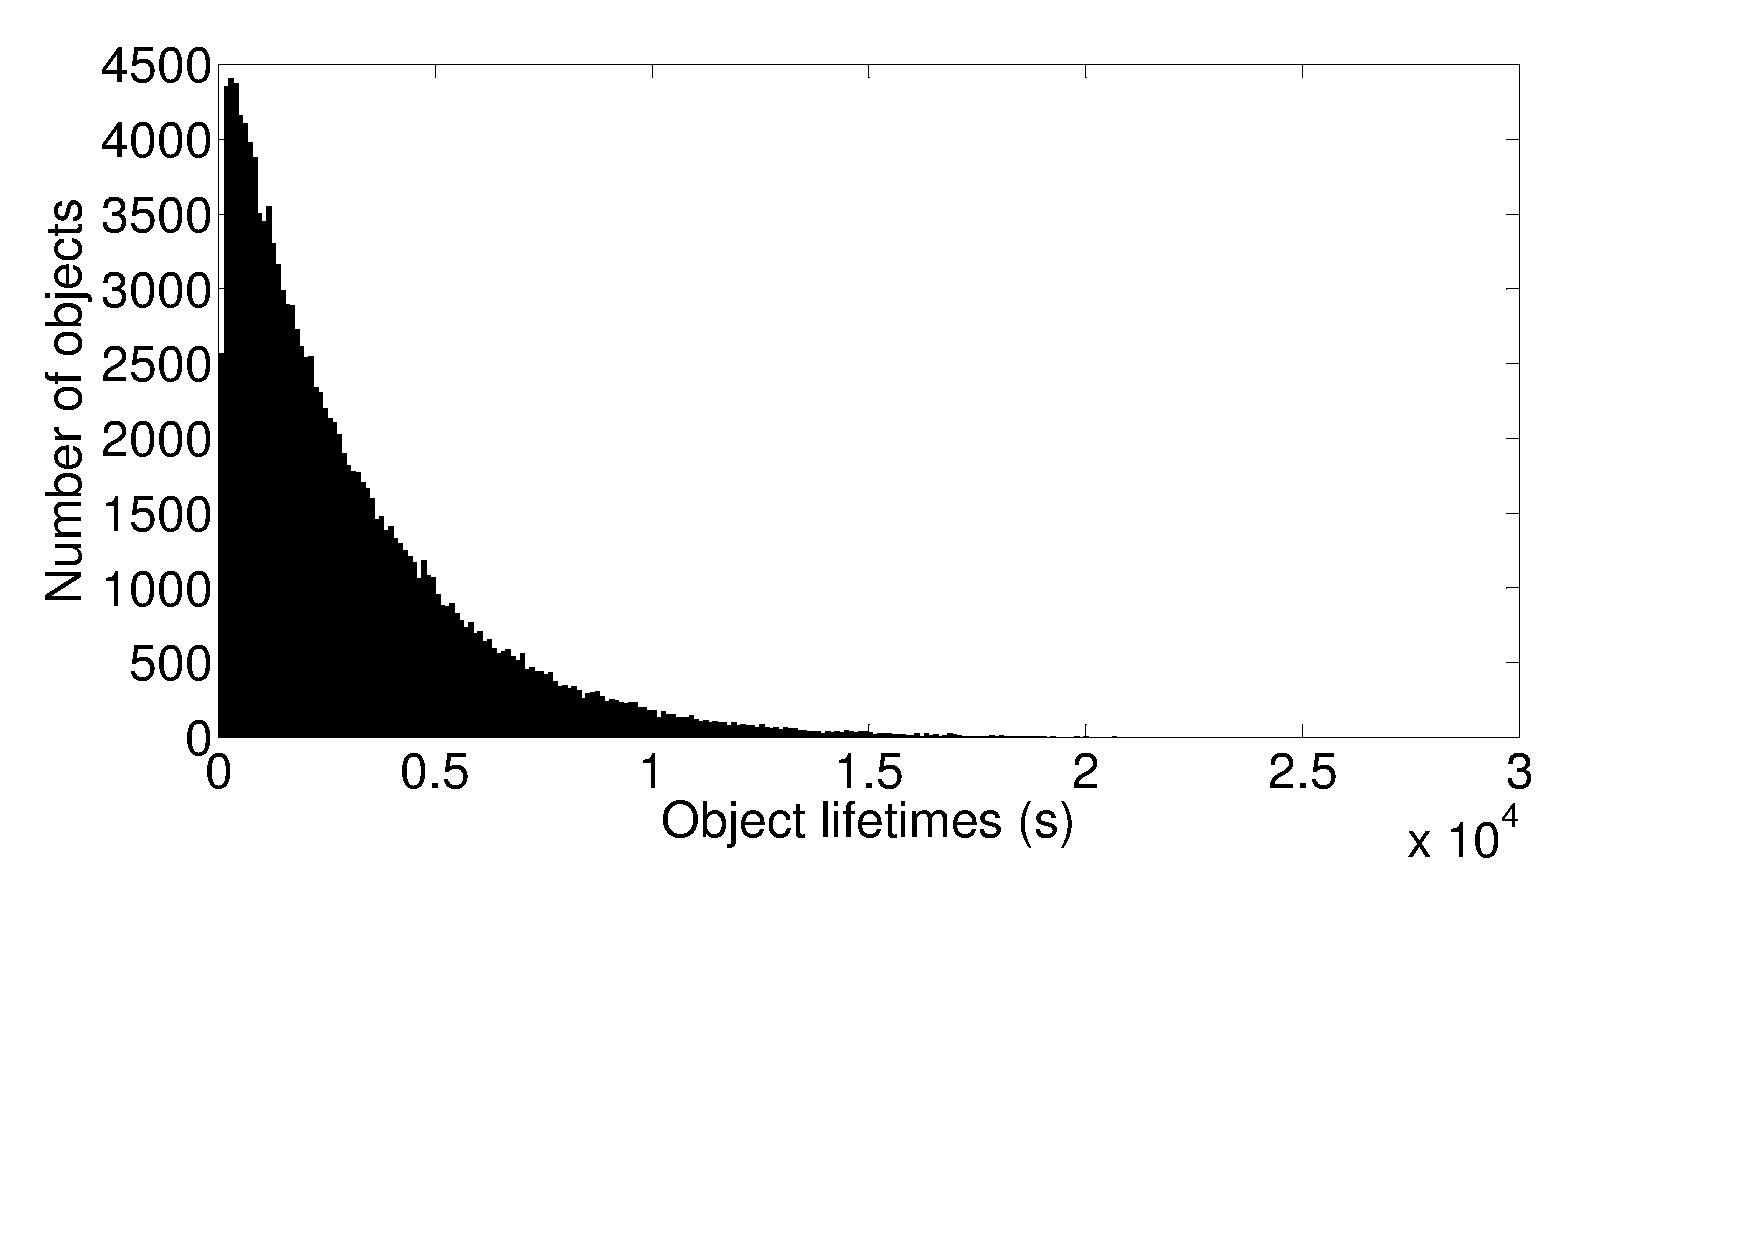
\includegraphics[clip=true, viewport=0.5cm 6.0cm 26.0cm 20.5cm, width=0.8\columnwidth]{object_lifetimes}
 \caption{Simulated object lifetime distribution}
 \label{fig_object_lifetimes}
\end{figure}
%
This shows that although expected object lifetimes can be accurately predicted, actual object lifetimes can vary greatly from the mean and can be much longer than expected. The heavy-tailed distribution might be as a consequence of an effect that is not yet being modelled.

\section{Conclusion}
\label{conclusion}

A Markov chain that takes network size into account when predicting object lifetimes was presented in this paper. Results show that when the average network size is comparable to the required number of replicas, object lifetimes are significantly decreased.

The theoretical model was shown to be equivalent to a model that ignores network size, when the average network size is large, compared to the required number of replicas. The model was also shown to compare well to simulation, with mean values being almost equal.

Although lifetimes means of the model were found to match well with the simulation, the simulation data showed a large variance, with a heavy tailed distribution. This leads one to believe that some other effect exists that is not yet being modelled. Further research into the phenomenon is required.

%What remains to be done.

%\newpage
% use section* for acknowledgement
\ifCLASSOPTIONcompsoc
  % The Computer Society usually uses the plural form
  \section*{Acknowledgments}
\else
  % regular IEEE prefers the singular form
  \section*{Acknowledgment}
\fi

The financial assistance of MIH and the National Research Foundation (NRF) towards this research is hereby acknowledged. Opinions expressed and
conclusions arrived at, are those of the author and are not necessarily to be attributed to MIH or the NRF.

%\newpage
%\IEEEtriggeratref{43} %Balance the bibliography
\bibliographystyle{IEEEtran}
\bibliography{../BibTeX/P2P_MMOG}

% that's all folks
\end{document}
